\documentclass[../main.tex]{subfiles}

\begin{document}

\section{Existing descriptive frameworks}\label{sec:descriptive-framework}

\subsection{Infeasibility of using derivational syntax as a descriptive tool}\label{sec:generative-no-good}

Though Minimalism is the most prevalent framework in the generative enterprise, 
we should acknowledge that the framework is not a good choice for descriptive means \citep{dryer2006descriptive}, 
and more surface-oriented grammatical theories (``descriptive theory'' in Dryer's terms) are required. 
The ultimate reason is Minimalism tends to work with rather abstract and fine-grained features 
with lots of movements and spell-out related post-syntactic morphological processes, 
which is just the purpose of generative research but proves not suitable for language describing from sketch.
When faced with real-world data, 
it is technically impossible for linguists to immediately work out the right derivation process. 
To list a few representative cases:
\begin{itemize}
    \item  How to decide the correct derivation procedure of an ergative language, since 
    linguists are still debating about several possible mechanisms?
    \item How to describe subcagegorization? By selectional features as in Minimalist Grammar,
    or by \ac{dm}-like spellout-based mechanisms\citep{siddiqi2009syntax}?
    \item How to account for different NP word orders? Should we accept them as they are, or should we introduce 
    some movements without clear motivation \citep{cinque2005deriving} to derive them from a universal supine?
\end{itemize}
A lot more questions can be added to this list. We see that surface-based ``shallow'' analysis and fine-grained 
analysis are conflicting, and hence it is reasonable to adopt other frameworks for language description.

Compared to Minimalism, GB is less fine-grained and we can expect it may be a better descriptive theory,
and there are GB grammars about underdocumented languages, for example \citet{holmer1996parametric}. 
This work, however, has poor reputation in linguists 
who care more about grammar writing than so-called in-depth analysis \citep{van2007holistic}.
These linguists contribute the most to our knowledge about particular languages, 
and they tend to be anti-generativism. Their words should definitely be taken seriously.
The viewpoint taken in this book is we do need descriptive theories in lieu of Minimalism,
but this is for practical reasons discussed above.
The formal sides of these descriptive theories, as I discuss later in this chapter, 
are essentially the same as Minimalism.

The other theory frameworks -- for example TAG -- are much better at grammar writing. 
We do not need much explanation for the descriptive power \ac{blt} or \ac{cgel}. 
For dependency grammar, we have the Universal Dependency project, 
which uses a unified annotation rule to build a large, multi-linguistic treebank \citep{ud}.
For \ac{tag}, we also have the XTAG project. % TODO: more citation

So now we have a list of a few existing structure-based frameworks that are relevant to our discussions:
\begin{itemize}
    \item Minimalism, which works on 
    \item The traditional GB-style X-bar scheme
    \item \ac{tag}  % TODO
    \item Dependency grammars, which is frequently used in computational works.
    \item \ac{blt}, the framework used in most contemporary descriptive works.
    \item The grammatical framework used in \ac{cgel} \citep{cgel,pullum2008expressive}, which is generative-informed and yet remaining 
    context-free and insists some analysis quite different from contemporary Minimalism (e.g. 
    what is a head -- I will discuss these apparent disagreements later).
\end{itemize}
Their differences can be roughly summarized as \prettyref{tbl:framework-comparison}. 
The ``surface-based partition'' and ``find-grained analysis'' rows 
explain why Minimalism fails as a descriptive theory. 
Minimalism is optimized for the latter, 
which other grammatical frameworks simply ignore, and as a consequence, 
Minimalism fails in the former task.

An obvious question is why there are so many frameworks, each of which seems to make some sense. 
In the rest of \prettyref{sec:descriptive-framework}, 
I explain items in \prettyref{tbl:framework-comparison}, 
the strength and weakness of each framework, 
and how these differences are mostly just notational differences 
and are more about methodology instead of worldview. 
The grammatical framework I use in this book for descriptive works is a mixture of all these framework,
with plenty of discussions on how these frameworks are related.
This is a reasonable choice in my own point of view. 
\citet{jacques2021grammar}, for example, is a typical \ac{blt} grammar, 
but when it comes the coordination strategies in NPs, 
some GB-style X-bar trees are used (Figure 9.1 and 9.2).

\begin{table}
    \centering
    \caption{Comparison between different formalisms. The yellow color means the corresponding framework is 
    able to have the feature, but relevant discussions are rare in the literature.}
    \label{tbl:framework-comparison}
    \begin{tabular}{@{}ccccccc@{}}
        \toprule
        Feature                                                                    & Minimalism                                                                                                & GB                                                                                                               & TAG                       & \begin{tabular}[c]{@{}c@{}}Dependency \\ grammar\end{tabular}                       & BLT                                              & CGEL                      \\ \midrule
        \begin{tabular}[c]{@{}c@{}}Surface-based \\ segmentation\end{tabular}      & \cellcolor[HTML]{FE0000}-                                                                                 & \cellcolor[HTML]{F8FF00}\begin{tabular}[c]{@{}c@{}}Descriptive\\ works exist\\ but not good\end{tabular}         & \cellcolor[HTML]{67FD9A}+ & \cellcolor[HTML]{67FD9A}{\color[HTML]{333333} +}                                    & \cellcolor[HTML]{67FD9A}{\color[HTML]{333333} +} & \cellcolor[HTML]{67FD9A}+ \\
        \begin{tabular}[c]{@{}c@{}}Fine grained \\ analysis\end{tabular} & \cellcolor[HTML]{67FD9A}+                                                                                 & \cellcolor[HTML]{F8FF00} Cartography                                                                                        & \cellcolor[HTML]{FE0000}- & \cellcolor[HTML]{FE0000}-                                                           & \cellcolor[HTML]{FE0000}-                        & \cellcolor[HTML]{FE0000}- \\
        Large ``domains''                                                            & \cellcolor[HTML]{F8FF00}\begin{tabular}[c]{@{}c@{}}phase theory,\\ cartography,\\ etc.\end{tabular}       & \cellcolor[HTML]{67FD9A}+                                                                                        & \cellcolor[HTML]{67FD9A}+ & \cellcolor[HTML]{FE0000}-                                                           & \cellcolor[HTML]{67FD9A}+                        & \cellcolor[HTML]{67FD9A}+ \\
        \begin{tabular}[c]{@{}c@{}}Pre-compiled \\ constructions\end{tabular}      & \cellcolor[HTML]{F8FF00}\begin{tabular}[c]{@{}c@{}}Nanosyntax-\\ like lexicon\end{tabular}                & \cellcolor[HTML]{F8FF00}                                                                                         & \cellcolor[HTML]{67FD9A}+ & \cellcolor[HTML]{F8FF00}\begin{tabular}[c]{@{}c@{}}valency \\ analysis\end{tabular} & \cellcolor[HTML]{67FD9A}+                        & \cellcolor[HTML]{F8FF00}  \\
        Hierarchy details                                                          & \cellcolor[HTML]{67FD9A}+                                                                                 & \cellcolor[HTML]{67FD9A}+                                                                                        & \cellcolor[HTML]{67FD9A}+ & \cellcolor[HTML]{FE0000}-                                                           & \cellcolor[HTML]{FE0000}-                        & \cellcolor[HTML]{67FD9A}+ \\
        Dependencies                                                               & \cellcolor[HTML]{F8FF00}\begin{tabular}[c]{@{}c@{}}Through\\ DM-like\\ subcateg-\\ orization\end{tabular} & \cellcolor[HTML]{F8FF00}\begin{tabular}[c]{@{}c@{}}Through\\ notions\\ like\\ Spec-head\\ relations\end{tabular} & \cellcolor[HTML]{FE0000}- & \cellcolor[HTML]{67FD9A}+                                                           & \cellcolor[HTML]{67FD9A}+                        & \cellcolor[HTML]{67FD9A}+ \\ \bottomrule
        \end{tabular}
    \end{table}

\subsection{Equivalent formalism of Minimalism}

\begin{figure}
    \centering
    

\tikzset{every picture/.style={line width=0.75pt}} %set default line width to 0.75pt        

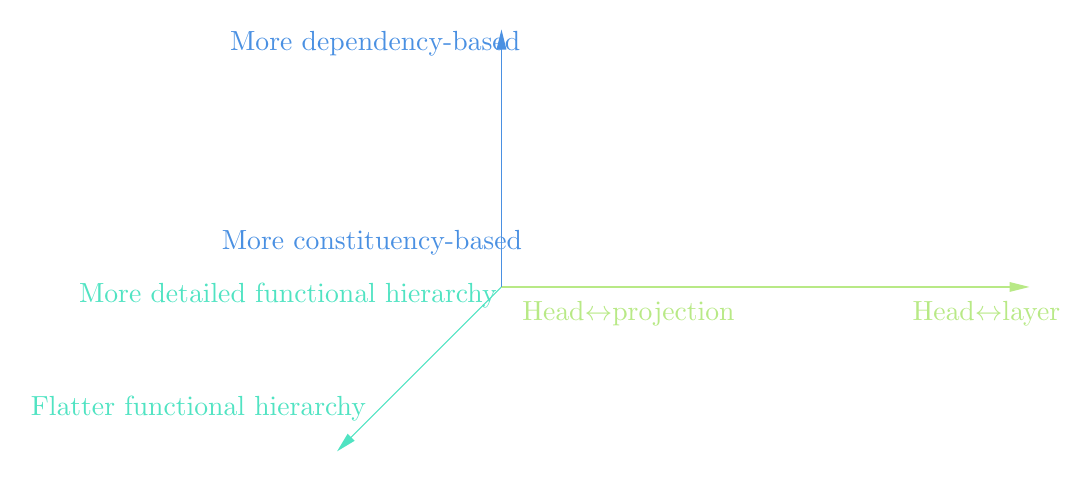
\begin{tikzpicture}[x=0.75pt,y=0.75pt,yscale=-0.8,xscale=0.8]
%uncomment if require: \path (0,536); %set diagram left start at 0, and has height of 536

%Straight Lines [id:da308608375613858] 
\draw [color={rgb, 255:red, 80; green, 227; blue, 194 }  ,draw opacity=1 ]   (323,220.81) -- (225.41,318.4) ;
\draw [shift={(224,319.81)}, rotate = 315] [fill={rgb, 255:red, 80; green, 227; blue, 194 }  ,fill opacity=1 ][line width=0.08]  [draw opacity=0] (12,-3) -- (0,0) -- (12,3) -- cycle    ;
%Straight Lines [id:da6591124487064512] 
\draw [color={rgb, 255:red, 184; green, 233; blue, 134 }  ,draw opacity=1 ]   (323,220.81) -- (639,220.81) ;
\draw [shift={(641,220.81)}, rotate = 180] [fill={rgb, 255:red, 184; green, 233; blue, 134 }  ,fill opacity=1 ][line width=0.08]  [draw opacity=0] (12,-3) -- (0,0) -- (12,3) -- cycle    ;
%Straight Lines [id:da7487030405468103] 
\draw [color={rgb, 255:red, 74; green, 144; blue, 226 }  ,draw opacity=1 ]   (323,220.81) -- (323,67.81) ;
\draw [shift={(323,65.81)}, rotate = 90] [fill={rgb, 255:red, 74; green, 144; blue, 226 }  ,fill opacity=1 ][line width=0.08]  [draw opacity=0] (12,-3) -- (0,0) -- (12,3) -- cycle    ;

% Text Node
\draw (158,65) node [anchor=north west][inner sep=0.75pt]  [color={rgb, 255:red, 74; green, 144; blue, 226 }  ,opacity=1 ] [align=left] {More dependency-based};
% Text Node
\draw (153,185) node [anchor=north west][inner sep=0.75pt]  [color={rgb, 255:red, 74; green, 144; blue, 226 }  ,opacity=1 ] [align=left] {More constituency-based};
% Text Node
\draw (67,217) node [anchor=north west][inner sep=0.75pt]  [color={rgb, 255:red, 80; green, 227; blue, 194 }  ,opacity=1 ] [align=left] {More detailed functional hierarchy};
% Text Node
\draw (38,285) node [anchor=north west][inner sep=0.75pt]  [color={rgb, 255:red, 80; green, 227; blue, 194 }  ,opacity=1 ] [align=left] {Flatter functional hierarchy};
% Text Node
\draw (334,228) node [anchor=north west][inner sep=0.75pt]  [color={rgb, 255:red, 184; green, 233; blue, 134 }  ,opacity=1 ] [align=left] {Head$\displaystyle \leftrightarrow $projection};
% Text Node
\draw (569,228) node [anchor=north west][inner sep=0.75pt]  [color={rgb, 255:red, 184; green, 233; blue, 134 }  ,opacity=1 ] [align=left] {Head$\displaystyle \leftrightarrow $layer};


\end{tikzpicture}

    \caption{Coordinates of equivalent Minimalism formalisms} 
    \label{fig:coordinate-minimalism}
\end{figure}

\prettyref{fig:coordinate-minimalism} gives a coordinate system which classifies possible equivalent formalisms
of Minimalism. \prettyref{fig:minimalism-mapping} illustrates how to explicitly build correspondence between 
different formalisms. In the following sections, I will talk about the three axes in these two figures. 

\begin{figure}
    \centering
    

\tikzset{every picture/.style={line width=0.75pt}} %set default line width to 0.75pt        

\begin{tikzpicture}[x=0.75pt,y=0.75pt,yscale=-0.8,xscale=0.8]
%uncomment if require: \path (0,681); %set diagram left start at 0, and has height of 681

%Straight Lines [id:da8350432578634659] 
\draw [color={rgb, 255:red, 74; green, 144; blue, 226 }  ,draw opacity=1 ]   (255,245) -- (255,186.48) ;
\draw [shift={(255,184.48)}, rotate = 90] [fill={rgb, 255:red, 74; green, 144; blue, 226 }  ,fill opacity=1 ][line width=0.08]  [draw opacity=0] (12,-3) -- (0,0) -- (12,3) -- cycle    ;
%Straight Lines [id:da12751595974157381] 
\draw    (276,319.52) -- (247,333.67) ;
%Straight Lines [id:da4633755411504048] 
\draw    (276,319.52) -- (305,333.67) ;
%Straight Lines [id:da6038585662271874] 
\draw    (305,356.67) -- (334,370.81) ;
%Straight Lines [id:da9621669176728602] 
\draw    (305,356.67) -- (276,370.81) ;
%Straight Lines [id:da22404281311176066] 
\draw    (334,397.81) -- (305,411.96) ;
%Straight Lines [id:da5964038780217018] 
\draw    (334,397.81) -- (363,411.96) ;
%Straight Lines [id:da29518019147428043] 
\draw    (247,281.52) -- (218,295.67) ;
%Straight Lines [id:da8313217199991596] 
\draw    (247,281.52) -- (276,295.67) ;

%Straight Lines [id:da6794750732287518] 
\draw [color={rgb, 255:red, 184; green, 233; blue, 134 }  ,draw opacity=1 ]   (351,322.81) -- (479,322.81) ;
\draw [shift={(481,322.81)}, rotate = 180] [fill={rgb, 255:red, 184; green, 233; blue, 134 }  ,fill opacity=1 ][line width=0.08]  [draw opacity=0] (12,-3) -- (0,0) -- (12,3) -- cycle    ;
%Straight Lines [id:da6367630865324176] 
\draw [color={rgb, 255:red, 80; green, 227; blue, 194 }  ,draw opacity=1 ]   (219,450.33) -- (165.75,503.59) ;
\draw [shift={(164.33,505)}, rotate = 315] [fill={rgb, 255:red, 80; green, 227; blue, 194 }  ,fill opacity=1 ][line width=0.08]  [draw opacity=0] (12,-3) -- (0,0) -- (12,3) -- cycle    ;
%Curve Lines [id:da06681999455732557] 
\draw [color={rgb, 255:red, 0; green, 0; blue, 0 }  ,draw opacity=1 ]   (247,82.48) .. controls (249.97,21.1) and (205.9,17.55) .. (200.16,80.55) ;
\draw [shift={(200,82.48)}, rotate = 274.4] [fill={rgb, 255:red, 0; green, 0; blue, 0 }  ,fill opacity=1 ][line width=0.08]  [draw opacity=0] (12,-3) -- (0,0) -- (12,3) -- cycle    ;
%Curve Lines [id:da9010875284671609] 
\draw [color={rgb, 255:red, 0; green, 0; blue, 0 }  ,draw opacity=1 ]   (252,82.48) .. controls (254.96,21.41) and (289.93,38.93) .. (294.8,81.52) ;
\draw [shift={(295,83.48)}, rotate = 264.81] [fill={rgb, 255:red, 0; green, 0; blue, 0 }  ,fill opacity=1 ][line width=0.08]  [draw opacity=0] (12,-3) -- (0,0) -- (12,3) -- cycle    ;
%Curve Lines [id:da47726983599244965] 
\draw [color={rgb, 255:red, 0; green, 0; blue, 0 }  ,draw opacity=1 ]   (304,81.48) .. controls (311.88,30.26) and (334.31,39.19) .. (338.81,81.52) ;
\draw [shift={(339,83.48)}, rotate = 264.81] [fill={rgb, 255:red, 0; green, 0; blue, 0 }  ,fill opacity=1 ][line width=0.08]  [draw opacity=0] (12,-3) -- (0,0) -- (12,3) -- cycle    ;
%Straight Lines [id:da8683620573651061] 
\draw    (158,574.52) -- (129,588.67) ;
%Straight Lines [id:da9777039126657969] 
\draw    (158,574.52) -- (187,588.67) ;
%Straight Lines [id:da8447403595321143] 
\draw    (583,319.52) -- (554,333.67) ;
%Straight Lines [id:da44472664370190573] 
\draw    (583,319.52) -- (612,333.67) ;
%Straight Lines [id:da546029464490396] 
\draw    (612,356.67) -- (641,370.81) ;
%Straight Lines [id:da25880810260479525] 
\draw    (612,356.67) -- (583,370.81) ;
%Straight Lines [id:da22632049791342013] 
\draw    (641,397.81) -- (612,411.96) ;
%Straight Lines [id:da2708332831470359] 
\draw    (641,397.81) -- (670,411.96) ;
%Straight Lines [id:da565274229303256] 
\draw    (554,281.52) -- (525,295.67) ;
%Straight Lines [id:da22642754581436475] 
\draw    (554,281.52) -- (583,295.67) ;
%Curve Lines [id:da506914942091861] 
\draw    (149,111.15) .. controls (160.94,169.85) and (247.13,184) .. (250.95,110.26) ;
\draw [shift={(251,109.15)}, rotate = 92.29] [fill={rgb, 255:red, 0; green, 0; blue, 0 }  ][line width=0.08]  [draw opacity=0] (12,-3) -- (0,0) -- (12,3) -- cycle    ;
%Straight Lines [id:da7103129253762701] 
\draw [color={rgb, 255:red, 184; green, 233; blue, 134 }  ,draw opacity=1 ]   (367,81.81) -- (468,81.81) ;
\draw [shift={(470,81.81)}, rotate = 180] [fill={rgb, 255:red, 184; green, 233; blue, 134 }  ,fill opacity=1 ][line width=0.08]  [draw opacity=0] (12,-3) -- (0,0) -- (12,3) -- cycle    ;
\draw [shift={(365,81.81)}, rotate = 0] [fill={rgb, 255:red, 184; green, 233; blue, 134 }  ,fill opacity=1 ][line width=0.08]  [draw opacity=0] (12,-3) -- (0,0) -- (12,3) -- cycle    ;
%Curve Lines [id:da597831463173695] 
\draw [color={rgb, 255:red, 0; green, 0; blue, 0 }  ,draw opacity=1 ]   (690,116.15) .. controls (667.12,144.01) and (589.78,173.85) .. (558.47,112.08) ;
\draw [shift={(558,111.15)}, rotate = 63.8] [fill={rgb, 255:red, 0; green, 0; blue, 0 }  ,fill opacity=1 ][line width=0.08]  [draw opacity=0] (12,-3) -- (0,0) -- (12,3) -- cycle    ;
%Curve Lines [id:da9028213106273151] 
\draw [color={rgb, 255:red, 0; green, 0; blue, 0 }  ,draw opacity=1 ]   (694,78.15) .. controls (671.35,24.96) and (652.57,41.62) .. (648.19,81.64) ;
\draw [shift={(648,83.48)}, rotate = 275.53] [fill={rgb, 255:red, 0; green, 0; blue, 0 }  ,fill opacity=1 ][line width=0.08]  [draw opacity=0] (12,-3) -- (0,0) -- (12,3) -- cycle    ;
%Curve Lines [id:da6504393632480485] 
\draw [color={rgb, 255:red, 0; green, 0; blue, 0 }  ,draw opacity=1 ]   (704,77.15) .. controls (711.96,25.41) and (597.16,-29.3) .. (598.96,82.45) ;
\draw [shift={(599,84.15)}, rotate = 268.49] [fill={rgb, 255:red, 0; green, 0; blue, 0 }  ,fill opacity=1 ][line width=0.08]  [draw opacity=0] (12,-3) -- (0,0) -- (12,3) -- cycle    ;
%Curve Lines [id:da09829751807839493] 
\draw    (503.13,114.2) .. controls (541.33,213.66) and (656.45,189.41) .. (701,116.15) ;
\draw [shift={(502,111.15)}, rotate = 70.24] [fill={rgb, 255:red, 0; green, 0; blue, 0 }  ][line width=0.08]  [draw opacity=0] (12,-3) -- (0,0) -- (12,3) -- cycle    ;
%Straight Lines [id:da530044878478577] 
\draw [color={rgb, 255:red, 74; green, 144; blue, 226 }  ,draw opacity=1 ]   (591,256) -- (591,197.48) ;
\draw [shift={(591,195.48)}, rotate = 90] [fill={rgb, 255:red, 74; green, 144; blue, 226 }  ,fill opacity=1 ][line width=0.08]  [draw opacity=0] (12,-3) -- (0,0) -- (12,3) -- cycle    ;
%Straight Lines [id:da17675280085880618] 
\draw    (131,537.52) -- (102,551.67) ;
%Straight Lines [id:da5903649030458693] 
\draw    (131,537.52) -- (160,551.67) ;
%Straight Lines [id:da22079682147404922] 
\draw    (535,574.52) -- (506,588.67) ;
%Straight Lines [id:da9029576654459877] 
\draw    (535,574.52) -- (564,588.67) ;
%Straight Lines [id:da1925387302840138] 
\draw    (508,537.52) -- (479,551.67) ;
%Straight Lines [id:da101307011931842] 
\draw    (508,537.52) -- (537,551.67) ;
%Straight Lines [id:da17160787754640627] 
\draw [color={rgb, 255:red, 184; green, 233; blue, 134 }  ,draw opacity=1 ]   (288,595.81) -- (416,595.81) ;
\draw [shift={(418,595.81)}, rotate = 180] [fill={rgb, 255:red, 184; green, 233; blue, 134 }  ,fill opacity=1 ][line width=0.08]  [draw opacity=0] (12,-3) -- (0,0) -- (12,3) -- cycle    ;
%Straight Lines [id:da8779914022363882] 
\draw [color={rgb, 255:red, 80; green, 227; blue, 194 }  ,draw opacity=1 ]   (622,460.33) -- (568.75,513.59) ;
\draw [shift={(567.33,515)}, rotate = 315] [fill={rgb, 255:red, 80; green, 227; blue, 194 }  ,fill opacity=1 ][line width=0.08]  [draw opacity=0] (12,-3) -- (0,0) -- (12,3) -- cycle    ;
%Straight Lines [id:da3995619192925306] 
\draw [color={rgb, 255:red, 80; green, 227; blue, 194 }  ,draw opacity=1 ]   (130,151.33) -- (76.75,204.59) ;
\draw [shift={(75.33,206)}, rotate = 315] [fill={rgb, 255:red, 80; green, 227; blue, 194 }  ,fill opacity=1 ][line width=0.08]  [draw opacity=0] (12,-3) -- (0,0) -- (12,3) -- cycle    ;
%Straight Lines [id:da989139903952883] 
\draw [color={rgb, 255:red, 74; green, 144; blue, 226 }  ,draw opacity=1 ]   (74,498) -- (74,393.48) ;
\draw [shift={(74,391.48)}, rotate = 90] [fill={rgb, 255:red, 74; green, 144; blue, 226 }  ,fill opacity=1 ][line width=0.08]  [draw opacity=0] (12,-3) -- (0,0) -- (12,3) -- cycle    ;
%Curve Lines [id:da7984911867977953] 
\draw [color={rgb, 255:red, 0; green, 0; blue, 0 }  ,draw opacity=1 ]   (15,300.48) .. controls (14.01,212.59) and (133.79,212.15) .. (126.13,300.15) ;
\draw [shift={(126,301.48)}, rotate = 275.75] [fill={rgb, 255:red, 0; green, 0; blue, 0 }  ,fill opacity=1 ][line width=0.08]  [draw opacity=0] (12,-3) -- (0,0) -- (12,3) -- cycle    ;
%Curve Lines [id:da07667237326010312] 
\draw [color={rgb, 255:red, 0; green, 0; blue, 0 }  ,draw opacity=1 ]   (105,298.48) .. controls (107.97,237.1) and (60.95,237.47) .. (55.16,300.55) ;
\draw [shift={(55,302.48)}, rotate = 274.4] [fill={rgb, 255:red, 0; green, 0; blue, 0 }  ,fill opacity=1 ][line width=0.08]  [draw opacity=0] (12,-3) -- (0,0) -- (12,3) -- cycle    ;

% Text Node
\draw (192,88.55) node [anchor=north west][inner sep=0.75pt]   [align=left] {XP};
% Text Node
\draw (250,88.55) node [anchor=north] [inner sep=0.75pt]  [color={rgb, 255:red, 0; green, 0; blue, 0 }  ,opacity=1 ] [align=left] {F1};
% Text Node
\draw (293,88.55) node [anchor=north] [inner sep=0.75pt]  [color={rgb, 255:red, 0; green, 0; blue, 0 }  ,opacity=1 ] [align=left] {F2};
% Text Node
\draw (339,88.55) node [anchor=north] [inner sep=0.75pt]   [align=left] {√Y};
% Text Node
\draw (220,12) node [anchor=north west][inner sep=0.75pt]  [color={rgb, 255:red, 0; green, 0; blue, 0 }  ,opacity=1 ] [align=left] {1};
% Text Node
\draw (264,20) node [anchor=north west][inner sep=0.75pt]  [color={rgb, 255:red, 0; green, 0; blue, 0 }  ,opacity=1 ] [align=left] {2};
% Text Node
\draw (158,571.52) node [anchor=south] [inner sep=0.75pt]   [align=left] {$>$};
% Text Node
\draw (129,591.67) node [anchor=north] [inner sep=0.75pt]   [align=left] {XP};
% Text Node
\draw (187,591.67) node [anchor=north] [inner sep=0.75pt]   [align=left] {Y$\displaystyle _{\text{[F1, F2]}}$};
% Text Node
\draw (276,316.52) node [anchor=south] [inner sep=0.75pt]   [align=left] {$>$};
% Text Node
\draw (247,336.67) node [anchor=north] [inner sep=0.75pt]   [align=left] {XP};
% Text Node
\draw (305,336.67) node [anchor=north] [inner sep=0.75pt]   [align=left] {$<$};
% Text Node
\draw (276,373.81) node [anchor=north] [inner sep=0.75pt]   [align=left] {F1};
% Text Node
\draw (334,373.81) node [anchor=north] [inner sep=0.75pt]   [align=left] {$<$};
% Text Node
\draw (305,414.96) node [anchor=north] [inner sep=0.75pt]   [align=left] {F2};
% Text Node
\draw (363,414.96) node [anchor=north] [inner sep=0.75pt]   [align=left] {√Y};
% Text Node
\draw (247,278.52) node [anchor=south] [inner sep=0.75pt]   [align=left] {$<$};
% Text Node
\draw (218,298.67) node [anchor=north] [inner sep=0.75pt]   [align=left] {F0};
% Text Node
\draw (583,316.52) node [anchor=south] [inner sep=0.75pt]   [align=left] {$>$};
% Text Node
\draw (554,336.67) node [anchor=north] [inner sep=0.75pt]   [align=left] {XP};
% Text Node
\draw (612,336.67) node [anchor=north] [inner sep=0.75pt]   [align=left] {$>$};
% Text Node
\draw (583,373.81) node [anchor=north] [inner sep=0.75pt]   [align=left] {F1};
% Text Node
\draw (641,373.81) node [anchor=north] [inner sep=0.75pt]   [align=left] {$>$};
% Text Node
\draw (612,414.96) node [anchor=north] [inner sep=0.75pt]   [align=left] {F2};
% Text Node
\draw (670,414.96) node [anchor=north] [inner sep=0.75pt]   [align=left] {√Y};
% Text Node
\draw (554,278.52) node [anchor=south] [inner sep=0.75pt]   [align=left] {$>$};
% Text Node
\draw (525,298.67) node [anchor=north] [inner sep=0.75pt]   [align=left] {F0};
% Text Node
\draw (147,88.48) node [anchor=north] [inner sep=0.75pt]  [color={rgb, 255:red, 0; green, 0; blue, 0 }  ,opacity=1 ] [align=left] {F0};
% Text Node
\draw (545,88.55) node [anchor=north west][inner sep=0.75pt]   [align=left] {XP};
% Text Node
\draw (603,88.55) node [anchor=north] [inner sep=0.75pt]  [color={rgb, 255:red, 0; green, 0; blue, 0 }  ,opacity=1 ] [align=left] {F1};
% Text Node
\draw (646,88.55) node [anchor=north] [inner sep=0.75pt]  [color={rgb, 255:red, 0; green, 0; blue, 0 }  ,opacity=1 ] [align=left] {F2};
% Text Node
\draw (692,88.55) node [anchor=north] [inner sep=0.75pt]   [align=left] {√Y};
% Text Node
\draw (582,160) node [anchor=north west][inner sep=0.75pt]  [color={rgb, 255:red, 0; green, 0; blue, 0 }  ,opacity=1 ] [align=left] {1};
% Text Node
\draw (603,8) node [anchor=north west][inner sep=0.75pt]  [color={rgb, 255:red, 0; green, 0; blue, 0 }  ,opacity=1 ] [align=left] {3};
% Text Node
\draw (500,88.48) node [anchor=north] [inner sep=0.75pt]  [color={rgb, 255:red, 0; green, 0; blue, 0 }  ,opacity=1 ] [align=left] {F0};
% Text Node
\draw (606,128) node [anchor=north west][inner sep=0.75pt]  [color={rgb, 255:red, 0; green, 0; blue, 0 }  ,opacity=1 ] [align=left] {2};
% Text Node
\draw (640,43) node [anchor=north west][inner sep=0.75pt]  [color={rgb, 255:red, 0; green, 0; blue, 0 }  ,opacity=1 ] [align=left] {4};
% Text Node
\draw (370,29) node [anchor=north west][inner sep=0.75pt]  [color={rgb, 255:red, 184; green, 233; blue, 134 }  ,opacity=1 ] [align=left] {moving the end of the arrow \\within the same layer};
% Text Node
\draw (377,341) node [anchor=north west][inner sep=0.75pt]  [color={rgb, 255:red, 184; green, 233; blue, 134 }  ,opacity=1 ] [align=left] {flip $>$ and $<$};
% Text Node
\draw (270,190) node [anchor=north west][inner sep=0.75pt]  [color={rgb, 255:red, 74; green, 144; blue, 226 }  ,opacity=1 ] [align=left] {draw dependency line between \\the head and its dependents};
% Text Node
\draw (312,462.15) node [anchor=north west][inner sep=0.75pt]  [color={rgb, 255:red, 80; green, 227; blue, 194 }  ,opacity=1 ] [align=left] {collapse a functional \\projection span};
% Text Node
\draw (131,534.52) node [anchor=south] [inner sep=0.75pt]   [align=left] {$<$};
% Text Node
\draw (102,554.67) node [anchor=north] [inner sep=0.75pt]   [align=left] {F0};
% Text Node
\draw (535,571.52) node [anchor=south] [inner sep=0.75pt]   [align=left] {$>$};
% Text Node
\draw (506,591.67) node [anchor=north] [inner sep=0.75pt]   [align=left] {XP};
% Text Node
\draw (564,591.67) node [anchor=north] [inner sep=0.75pt]   [align=left] {Y$\displaystyle _{\text{[F1, F2]}}$};
% Text Node
\draw (508,534.52) node [anchor=south] [inner sep=0.75pt]   [align=left] {$>$};
% Text Node
\draw (479,554.67) node [anchor=north] [inner sep=0.75pt]   [align=left] {F0};
% Text Node
\draw (314,571) node [anchor=north west][inner sep=0.75pt]  [color={rgb, 255:red, 184; green, 233; blue, 134 }  ,opacity=1 ] [align=left] {flip $>$ and $<$};
% Text Node
\draw (14,96.15) node [anchor=north west][inner sep=0.75pt]  [color={rgb, 255:red, 80; green, 227; blue, 194 }  ,opacity=1 ] [align=left] {combine several\\dependency \\lines};
% Text Node
\draw (64,315.67) node [anchor=north] [inner sep=0.75pt]   [align=left] {XP};
% Text Node
\draw (122,313.17) node [anchor=north] [inner sep=0.75pt]   [align=left] {Y$\displaystyle _{\text{[F1, F2]}}$};
% Text Node
\draw (16,315.67) node [anchor=north] [inner sep=0.75pt]   [align=left] {F0};


\end{tikzpicture}

    \caption{Mapping between equivalent formalisms}
    \label{fig:minimalism-mapping}
\end{figure}

There is yet a final coordinate of formalisms equivalent to Minimalism 
beside what is shown in \prettyref{fig:minimalism-mapping}: 
pre-compiled trees (read: ``construction''). 
I will not talk about this topic too much in this section, 
because there is no single way to routinize Minimalism derivations, 
so routinization cannot be easily represented 
by adding a more coordinate into \prettyref{fig:coordinate-minimalism}.

\subsubsection{Dependency vs constituency}\label{sec:minimalist-dependency}

Dependency grammars are often said to be alternatives to constituency grammars.
This is a quite weird claim, since they are better described as \emph{dual} to each other.
It has already been demonstrated that there are dependency structures in Minimalism \citep{boston2009dependency},
and Minimalism, under certain adaptation, is equivalent to a dependency grammar \citep{osborne2011bare}.
This should not surprise anyone, since there have long been tools converting one into another in old-fashioned NLP.
It is actually also possible to mix constituency grammar and dependency grammar 
\cite{kahane-mazziotta-2015-syntactic}, in which a dependent ark may point to a constituent and not necessarily a word.

\subsubsection{Divergent standards of constituency: how to divide a large unit}\label{sec:divergent-standard-constituency-segmentation}

Note that in Distributed Morphology, a word -- a bundle of several features spelt-out together -- 
is a \emph{span} and not a constituent in the generative sense, 
and yet in lexicalist Minimalism, people recognize it as a construction. 
This helps to settle the bracketing dilemma in immediate constituency analysis.

So now we can see there is no conflict 
between the binary branching definition of \term{verb phrase} as Aux plus V plus NP_{\text{object}} 
and the \ac{blt} definition of verb phrase, which does not include the object NP. 
A good choice is to use the term \term{verb complex} to denote the verb phrase in the \ac{blt} sense \citep[among others]{Wilbur2014,Friesen2017}.

\subsubsection{Divergent standards of constituency: how flat the tree is}

The fact that the relative height of dependency relations are never considered 
in standard dependency grammars raises yet another issue about 
how flat the syntax \emph{constituency} tree should be,
since we can map a dependency grammar without any marking of relative height of dependency relations 
(i.e. a dependency grammar which does not have labels 1, 2, \dots on dependency arcs as in \prettyref{fig:minimalism-mapping})
into a constituency grammar with flat trees. 
It is kind of strange to talk about flat trees in a theory equivalent to Minimalism, 
but recall that in lexicalist Minimalism, 
a terminal node in a syntactic tree can have unrestrictedly large feature bundles i.e. unrestricted branching, 
and since we know lexicalist Minimalism can be seen as an equivalent formalism of DM-like Minimalism, 
it is nature to ask whether unrestricted branching for \emph{all} kinds of nodes 
-- not just feature nodes -- also gives an equivalent grammar class to the grammar class allowed in Minimalism.

Take the tree structure of a simple clause as an example. 
In \ac{blt}, Dixon accuses the binary division between 
the subject and the predicate as harmful (without providing much argumentation about it), but when discussing 
topic and pivots, he distinguishes the subject (in accusative languages, of course) from other arguments and regards it as having a somehow more 
prominent position. The arguments are licensed by the verb and have dependency relations with the verb. 
Introducing a position of pivot (or subject in accusative languages) besides the notion of deep S, A and O 
of course means introducing a layer of construction built \emph{upon} the argument structure layer
about ``the obligatory and syntactically codified topic'', 
which, in generative terms, is just the TP layer. It is of course possible to draw a syntactic tree 
with a quite flat clause structure and explain that ``the subject somehow has a higher position'', 
but this is eventually the same as the binary branch approach in Minimalism.

\begin{figure}
    \centering
    

\tikzset{every picture/.style={line width=0.75pt}} %set default line width to 0.75pt        

\begin{tikzpicture}[x=0.75pt,y=0.75pt,yscale=-1,xscale=1]
%uncomment if require: \path (0,577); %set diagram left start at 0, and has height of 577

%Straight Lines [id:da3571919269318433] 
\draw    (294,104.56) -- (265,118.71) ;
%Straight Lines [id:da6561258080060619] 
\draw    (294,104.56) -- (323,118.71) ;
%Straight Lines [id:da06898664551834899] 
\draw    (321,147.48) -- (358,165.85) ;
%Straight Lines [id:da8075756397517635] 
\draw    (321,147.48) -- (285,164.48) ;
%Straight Lines [id:da41665955900317875] 
\draw    (358,192.85) -- (329,207) ;
%Straight Lines [id:da9079604504645364] 
\draw    (358,192.85) -- (387,207) ;
%Straight Lines [id:da7478179026703973] 
\draw    (239,54.48) -- (187,78.71) ;
%Straight Lines [id:da456511156570109] 
\draw    (239,54.48) -- (290,78.71) ;
%Straight Lines [id:da5715409936346081] 
\draw    (386,238.71) -- (415,252.85) ;
%Straight Lines [id:da9144092856943298] 
\draw    (386,238.71) -- (357,252.85) ;
%Straight Lines [id:da550303334673411] 
\draw    (415,276.85) -- (386,291) ;
%Straight Lines [id:da5505916969954645] 
\draw    (415,276.85) -- (444,291) ;
%Straight Lines [id:da848474007635855] 
\draw    (443,322.71) -- (472,336.85) ;
%Straight Lines [id:da4690731977225433] 
\draw    (443,322.71) -- (414,336.85) ;
%Shape: Ellipse [id:dp6349484937583538] 
\draw   (241,110.35) .. controls (251.36,101.76) and (275.54,113.86) .. (294.99,137.36) .. controls (314.45,160.86) and (321.82,186.87) .. (311.45,195.45) .. controls (301.08,204.03) and (276.91,191.94) .. (257.45,168.44) .. controls (237.99,144.94) and (230.63,118.93) .. (241,110.35) -- cycle ;
%Curve Lines [id:da13670515659331373] 
\draw [color={rgb, 255:red, 155; green, 155; blue, 155 }  ,draw opacity=1 ]   (254,163.48) .. controls (208.46,148.63) and (205.06,160.24) .. (182.68,201.73) ;
\draw [shift={(182,203)}, rotate = 298.41] [fill={rgb, 255:red, 155; green, 155; blue, 155 }  ,fill opacity=1 ][line width=0.08]  [draw opacity=0] (12,-3) -- (0,0) -- (12,3) -- cycle    ;
%Shape: Ellipse [id:dp6152794315221408] 
\draw   (318.95,190.86) .. controls (347.52,155.06) and (423.21,167.96) .. (488.01,219.67) .. controls (552.81,271.38) and (582.18,342.33) .. (553.61,378.13) .. controls (525.04,413.93) and (449.35,401.03) .. (384.55,349.32) .. controls (319.75,297.61) and (290.38,226.67) .. (318.95,190.86) -- cycle ;
%Curve Lines [id:da73255009866522] 
\draw  [dash pattern={on 4.5pt off 4.5pt}]  (337.8,269.11) .. controls (299.4,323.15) and (369.03,405.1) .. (471,367.48) ;
\draw [shift={(339,267.48)}, rotate = 127.21] [fill={rgb, 255:red, 0; green, 0; blue, 0 }  ][line width=0.08]  [draw opacity=0] (12,-3) -- (0,0) -- (12,3) -- cycle    ;
%Curve Lines [id:da5371088007693434] 
\draw  [dash pattern={on 4.5pt off 4.5pt}]  (345.87,273.79) .. controls (342.98,323.87) and (342.8,336.72) .. (395,352.48) ;
\draw [shift={(346,271.48)}, rotate = 93.3] [fill={rgb, 255:red, 0; green, 0; blue, 0 }  ][line width=0.08]  [draw opacity=0] (12,-3) -- (0,0) -- (12,3) -- cycle    ;
%Shape: Ellipse [id:dp4170769301823447] 
\draw   (329,237.35) .. controls (339.36,228.76) and (356.94,232.88) .. (368.25,246.54) .. controls (379.56,260.21) and (380.33,278.24) .. (369.96,286.83) .. controls (359.59,295.41) and (342.02,291.29) .. (330.7,277.63) .. controls (319.39,263.96) and (318.63,245.93) .. (329,237.35) -- cycle ;
%Curve Lines [id:da8605216809412348] 
\draw [color={rgb, 255:red, 155; green, 155; blue, 155 }  ,draw opacity=1 ]   (324,266.48) .. controls (270.54,268.46) and (265.1,275.34) .. (210.66,259.95) ;
\draw [shift={(209,259.48)}, rotate = 15.95] [fill={rgb, 255:red, 155; green, 155; blue, 155 }  ,fill opacity=1 ][line width=0.08]  [draw opacity=0] (12,-3) -- (0,0) -- (12,3) -- cycle    ;
%Shape: Ellipse [id:dp9342228745072949] 
\draw   (133.13,175.12) .. controls (149.65,161.45) and (184.75,176.58) .. (211.52,208.92) .. controls (238.3,241.26) and (246.61,278.57) .. (230.09,292.24) .. controls (213.57,305.92) and (178.47,290.79) .. (151.7,258.44) .. controls (124.93,226.1) and (116.61,188.8) .. (133.13,175.12) -- cycle ;
%Curve Lines [id:da026296240479518618] 
\draw    (321,218.48) .. controls (214.08,221.45) and (186.55,154.83) .. (186.98,108.87) ;
\draw [shift={(187,107.48)}, rotate = 91.25] [fill={rgb, 255:red, 0; green, 0; blue, 0 }  ][line width=0.08]  [draw opacity=0] (12,-3) -- (0,0) -- (12,3) -- cycle    ;
%Shape: Ellipse [id:dp018559860692994645] 
\draw   (49,62.17) .. controls (126.16,-27.48) and (302.23,-2.43) .. (442.27,118.1) .. controls (582.31,238.64) and (633.28,409.02) .. (556.12,498.67) .. controls (478.96,588.31) and (302.89,563.27) .. (162.85,442.73) .. controls (22.81,322.19) and (-28.16,151.81) .. (49,62.17) -- cycle ;

% Text Node
\draw (294,101.56) node [anchor=south] [inner sep=0.75pt]   [align=left] {T'};
% Text Node
\draw (265,121.71) node [anchor=north] [inner sep=0.75pt]   [align=left] {Pres};
% Text Node
\draw (321,125.71) node [anchor=north] [inner sep=0.75pt]   [align=left] {AspP};
% Text Node
\draw (285,167.48) node [anchor=north] [inner sep=0.75pt]   [align=left] {Perf};
% Text Node
\draw (358,168.85) node [anchor=north] [inner sep=0.75pt]   [align=left] {$\displaystyle v$P};
% Text Node
\draw (329,210) node [anchor=north] [inner sep=0.75pt]   [align=left] {\st{I}};
% Text Node
\draw (387,210) node [anchor=north] [inner sep=0.75pt]   [align=left] {$\displaystyle v_{\text{Do}} '$};
% Text Node
\draw (239,51.48) node [anchor=south] [inner sep=0.75pt]   [align=left] {TP};
% Text Node
\draw (357,255.85) node [anchor=north] [inner sep=0.75pt]   [align=left] {Do};
% Text Node
\draw (415,255.85) node [anchor=north] [inner sep=0.75pt]   [align=left] {TransP};
% Text Node
\draw (386,294) node [anchor=north] [inner sep=0.75pt]   [align=left] {[the task]};
% Text Node
\draw (444,294) node [anchor=north] [inner sep=0.75pt]   [align=left] {Trans'};
% Text Node
\draw (414,339.85) node [anchor=north] [inner sep=0.75pt]   [align=left] {Trans};
% Text Node
\draw (187,81.71) node [anchor=north] [inner sep=0.75pt]   [align=left] {I};
% Text Node
\draw (450,339) node [anchor=north west][inner sep=0.75pt]   [align=left] {√COMPLETE};
% Text Node
\draw (468,237) node [anchor=north west][inner sep=0.75pt]   [align=left] {layer 1: \\deep \\argument \\structure};
% Text Node
\draw (165,205) node [anchor=north west][inner sep=0.75pt]   [align=left] {have};
% Text Node
\draw (153,240) node [anchor=north west][inner sep=0.75pt]   [align=left] {completed};
% Text Node
\draw (49,232) node [anchor=north west][inner sep=0.75pt]   [align=left] {verb phrase};
% Text Node
\draw (115,77) node [anchor=north west][inner sep=0.75pt]   [align=left] {layer 3:\\subject\\movement};
% Text Node
\draw (309,431) node [anchor=north west][inner sep=0.75pt]   [align=left] {layer 2:\\basic\\clause \\structure};


\end{tikzpicture}

    \caption{The derivation of \emph{I have completed my task} in Minimalism}
    \label{fig:complete-my-task-minimalism}
\end{figure}

Here I give an example of multi-branch trees that are equivalent to Minimalist ones.
Since it is hard to define Merge-like fine-grained primitive operations with multiple branching,
I will present a tree in a grammar working with routinized pre-compiled constructions, 
not Merge and a list of syntactic atoms. I will talk about routinization in detail in \prettyref{sec:routine}. 

Consider, for example, the derivational process shown in \prettyref{fig:complete-my-task-minimalism}.
This seems complicated because we are only allowed to use Merge and spellout, 
but we can certainly find three routinized processes: 
the first is to assemble the $v$P structure and to build the argument structure, 
the second is to add tense and aspect information and to spell out them as auxiliary verbs
(hence forming the ``verb phrase'' in the \ac{blt} sense), 
and the third is the A-movement of the subject.
If we work with these routines instead of Merge and spellout, 
we get the dependency arcs in \prettyref{fig:complete-my-task-dep}.
Dependency relations created in the three layers are labeled by three colors.
The deep argument structure is realized in the $v$P layer in the Minimalism derivation.
The clausal non-spatial settings (this is the terminology in \ac{blt}) are created in the TP layer.
The fact that in active clauses the A argument is the pivot is realized by the Spec-$v$P to Spec-TP A-movement.%
\footnote{One question here might be that layer 2 seems to be the T' projection, 
while layer 3 seems to be the Spec-TP position and EPP feature, 
but it seems strange that a construction routinizes an intermediate projection. 
But for the sake of conciseness, 
\prettyref{fig:complete-my-task-minimalism} is \emph{not} a true cartographic syntactic tree, 
and just as is the case with \ac{cgel} where 
a projection corresponding to N' in the classical X-bar theory is actually a maximal projection, 
so is T' in \prettyref{fig:complete-my-task-minimalism}.}

\begin{figure}
    \centering 
    

\tikzset{every picture/.style={line width=0.75pt}} %set default line width to 0.75pt        

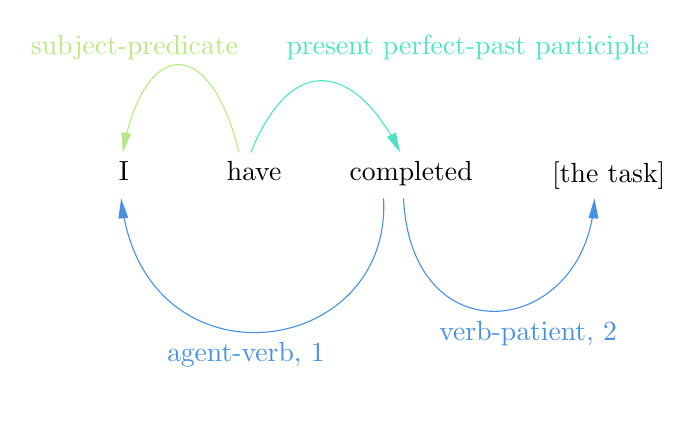
\begin{tikzpicture}[x=0.75pt,y=0.75pt,yscale=-0.8,xscale=0.8]
%uncomment if require: \path (0,300); %set diagram left start at 0, and has height of 300

%Curve Lines [id:da8298848597114246] 
\draw [color={rgb, 255:red, 74; green, 144; blue, 226 }  ,draw opacity=1 ]   (511.85,179.28) .. controls (505.89,260.1) and (401.95,273.83) .. (397,176.81) ;
\draw [shift={(512,176.81)}, rotate = 92.76] [fill={rgb, 255:red, 74; green, 144; blue, 226 }  ,fill opacity=1 ][line width=0.08]  [draw opacity=0] (12,-3) -- (0,0) -- (12,3) -- cycle    ;
%Curve Lines [id:da7977309817595222] 
\draw [color={rgb, 255:red, 74; green, 144; blue, 226 }  ,draw opacity=1 ]   (227.4,180.28) .. controls (242,293.42) and (389.95,273.83) .. (385,176.81) ;
\draw [shift={(227,176.81)}, rotate = 84.14] [fill={rgb, 255:red, 74; green, 144; blue, 226 }  ,fill opacity=1 ][line width=0.08]  [draw opacity=0] (12,-3) -- (0,0) -- (12,3) -- cycle    ;
%Curve Lines [id:da3756396013841674] 
\draw [color={rgb, 255:red, 80; green, 227; blue, 194 }  ,draw opacity=1 ]   (393.87,146.88) .. controls (368.83,97.77) and (330.61,86.11) .. (305,149.15) ;
\draw [shift={(395,149.15)}, rotate = 243.89] [fill={rgb, 255:red, 80; green, 227; blue, 194 }  ,fill opacity=1 ][line width=0.08]  [draw opacity=0] (12,-3) -- (0,0) -- (12,3) -- cycle    ;
%Curve Lines [id:da9846757481246158] 
\draw [color={rgb, 255:red, 184; green, 233; blue, 134 }  ,draw opacity=1 ]   (228.51,146.26) .. controls (240.2,83.84) and (279.29,74.29) .. (298,149.15) ;
\draw [shift={(228,149.15)}, rotate = 279.61] [fill={rgb, 255:red, 184; green, 233; blue, 134 }  ,fill opacity=1 ][line width=0.08]  [draw opacity=0] (12,-3) -- (0,0) -- (12,3) -- cycle    ;

% Text Node
\draw (224,153) node [anchor=north west][inner sep=0.75pt]   [align=left] {I};
% Text Node
\draw (289,153) node [anchor=north west][inner sep=0.75pt]   [align=left] {have};
% Text Node
\draw (363,153) node [anchor=north west][inner sep=0.75pt]   [align=left] {completed};
% Text Node
\draw (485,153) node [anchor=north west][inner sep=0.75pt]   [align=left] {[the task]};
% Text Node
\draw (417,249) node [anchor=north west][inner sep=0.75pt]  [color={rgb, 255:red, 74; green, 144; blue, 226 }  ,opacity=1 ] [align=left] {verb-patient, 2};
% Text Node
\draw (253,262) node [anchor=north west][inner sep=0.75pt]  [color={rgb, 255:red, 74; green, 144; blue, 226 }  ,opacity=1 ] [align=left] {agent-verb, 1};
% Text Node
\draw (325,77) node [anchor=north west][inner sep=0.75pt]  [color={rgb, 255:red, 80; green, 227; blue, 194 }  ,opacity=1 ] [align=left] {present perfect-past participle};
% Text Node
\draw (171,77) node [anchor=north west][inner sep=0.75pt]  [color={rgb, 255:red, 184; green, 233; blue, 134 }  ,opacity=1 ] [align=left] {subject-predicate};


\end{tikzpicture}

    \caption{The dependency relation created when deriving \emph{I have completed my task} in \ac{blt}}
    \label{fig:complete-my-task-dep}
\end{figure}

Now the problem is how can \prettyref{fig:complete-my-task-dep} be rephrased into a constituency tree 
which is multi-branch. After some reflection, it is easy to find that 
the \ac{blt} version of tree diagram shown in \prettyref{fig:complete-my-task-blt-1} is exactly what is wanted.
Every syntactic relation in the \ac{blt} tree diagram 
traces back to a dependency relation created by Merge. 
The grammatical relation between the auxiliary verb and the past participle is shown 
by combining these two into one unit, called the \emph{verb phrase} (in the \ac{blt} sense).
This is a \emph{span} in generative terms, being the newly added elements in the TP layer,
representing the non-spatial setting of the clause -- in this case it is ``present perfect''.
The argument structure \ac{blt} tree is realized by putting agent and patient labels to the arguments.
The pivot status of the agent is shown by the A label, 
which marks the agent NP and marks its pivot status at the same time.

Readers need additional knowledge put aside 
the tree diagram in \prettyref{fig:complete-my-task-blt-1}, which, essentially, 
means we need dependency relations not shown in the tree diagram.
This is the cost of rejection of fine-grained constituent structure: 
coexistence of flat trees and dependency relations is needed.

\begin{figure}
    \centering
    

\tikzset{every picture/.style={line width=0.75pt}} %set default line width to 0.75pt        

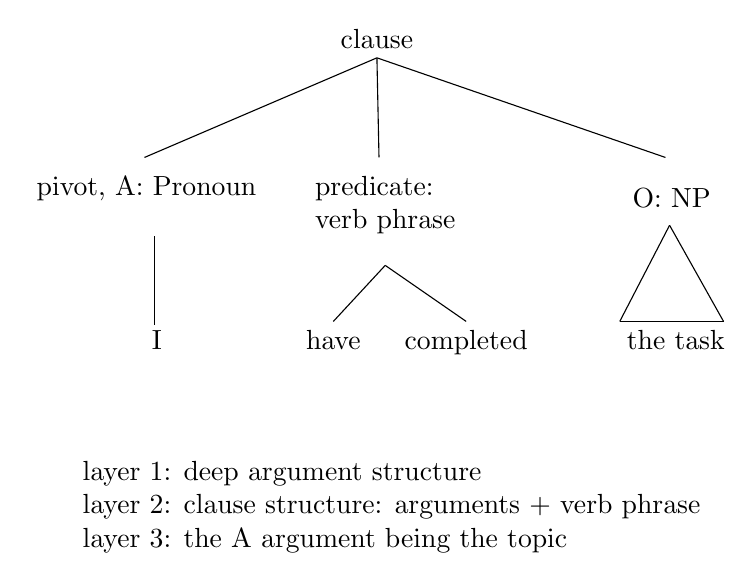
\begin{tikzpicture}[x=0.75pt,y=0.75pt,yscale=-1,xscale=1]
%uncomment if require: \path (0,390); %set diagram left start at 0, and has height of 390

%Straight Lines [id:da4161051988460063] 
\draw    (183,100.81) -- (71,148.81) ;
%Straight Lines [id:da36248311433047187] 
\draw    (187,200.81) -- (162,227.81) ;
%Straight Lines [id:da4439661314753782] 
\draw    (187,200.81) -- (226,227.81) ;
%Straight Lines [id:da36890954567869483] 
\draw    (300,227.81) -- (350,227.81) ;
%Straight Lines [id:da011342458373226894] 
\draw    (324,181.48) -- (300,227.81) ;
%Straight Lines [id:da5435200709744346] 
\draw    (324,181.48) -- (350,227.81) ;
%Straight Lines [id:da24568188379824396] 
\draw    (76,186.81) -- (76,229.48) ;
%Straight Lines [id:da3308532295080375] 
\draw    (183,100.81) -- (184,148.81) ;
%Straight Lines [id:da7487945318074942] 
\draw    (183,100.81) -- (322,148.81) ;

% Text Node
\draw (77,230.81) node [anchor=north] [inner sep=0.75pt]   [align=left] {I};
% Text Node
\draw (162,230.81) node [anchor=north] [inner sep=0.75pt]   [align=left] {have};
% Text Node
\draw (226,230.81) node [anchor=north] [inner sep=0.75pt]   [align=left] {completed};
% Text Node
\draw (327,230.81) node [anchor=north] [inner sep=0.75pt]   [align=left] {the task};
% Text Node
\draw (187,187) node [anchor=south] [inner sep=0.75pt]   [align=left] {predicate:\\verb phrase};
% Text Node
\draw (325,174) node [anchor=south] [inner sep=0.75pt]   [align=left] {O: NP};
% Text Node
\draw (15,157) node [anchor=north west][inner sep=0.75pt]   [align=left] {\begin{minipage}[lt]{83.56pt}\setlength\topsep{0pt}
\begin{center}
pivot, A: Pronoun
\end{center}

\end{minipage}};
% Text Node
\draw (183,97.81) node [anchor=south] [inner sep=0.75pt]   [align=left] {clause};
% Text Node
\draw (40,294) node [anchor=north west][inner sep=0.75pt]   [align=left] {layer 1: deep argument structure\\layer 2: clause structure: arguments + verb phrase\\layer 3: the A argument being the topic};


\end{tikzpicture}

    \caption{The tree diagram representation of \emph{I have completed my task} in \ac{blt}}
    \label{fig:complete-my-task-blt-1}
\end{figure}

A similar case where the loss of structural information in less fine-grained formalisms
is remended by adding additional dependency relations can be found in \ac{cgel} \citesec{5.14.1}, 
where the authors highlight the existence of \emph{indirect} complements, 
which are licensed by another dependent in the matrix phrase, 
and the dependency relation between an indirect complement and its licensor is not that 
transparent in \ac{cgel}'s phrase structure grammar.
In this case, additional dependency relations arise from rejection of invisible movements.

A further issue about the flatness of tree diagrams is how to describe the constituency order.
The flat-tree approach, which is used in \ac{blt} and also known as the functional theory of syntax,
views constituent order as a mean to mark the constituents,
in the same way case markers mark NPs.
For a SVO language like Chinese or English, for example, 
the \ac{blt} perspective is that the O argument is marked by 
the fact that it follows the predicator.
As Dixon points out, the constituent order is about surface realization and is largely arbitrary,
easily variable just like case marking strategies.
Thus, the generative papers trying to somehow ``derive'' the constituent order
seem to be all meaningless.%
\footnote{
    There is a widespread myth in functionalists that 
    generative linguistics try to demonstrate 
    all human languages have English-like underlying constituent orders.
    This myth is sometimes expressed via claims like 
    ``Chomsky is a language colonizer'' or 
    ``Chomsky tells us that all languages are European languages.''
    This myth has factual errors as well as misunderstanding of what generativism tries to do.
    The factual errors include 
    that in Minimalism, the S-structure v.s. D-structure distinction is canceled,
    and there is simply no such thing as English-like D-structures in contemporary generative syntax,
    that though some linguists assume a universal left-branching derivational order 
    or cartographic supine,
    which captures the essential idea of the old-fashioned D-structure,
    not all generative linguists insist on this universal supine \citep{wiltschko2014universal},
    and that even for those accepting the cartographic syntax completely,
    due to the Distributed Morphology-like lexical decomposition,
    the verb root may be in the rightmost position in the universal supine,
    which moves to its surface position by head movements in SVO languages,
    and hence the ``underlying constituent order'' (as functionalists call it)
    is better described as Japanese-like rather than English-like.
    In the Chomsky-as-language-colonizer logic, then,
    if a linguist does not a lexical decomposition approach, he or she is a language colonizer,
    and otherwise, he or she embraces diversity.
    This line of thinking is as absurd as it seems.
    The misunderstanding of what generativism is discussed hereafter.
}
The problem is this does not goes against the generative idea:
in generative syntax, movements which cause deviation 
from the trivial tree structure created by external Merge 
are driven by features, 
in the same way case marking is driven by features.
The movement-free template-based approach of syntax,
despite its apparent discrepancy with the contemporary generative approach,
describes a largely identical grammatical complexity class with the generative one:
``a feature attracts S to its surface position''
has nothing practically different from ``a feature is marked by inserting S to its surface position''.
What, then, does the invisible and chaotic features and derivations add to our understanding of language?
What they add to our understanding of language 
is that the variation of constituency order is \emph{not} that free:
certain antisymmetric effects can be observed,
which do not have clear functional explanation \citep{cinque2014typological}.
A right-branching Merge-based analysis extracts these observations in the notation,
and hence is helpful when doing both internal and cross-linguistic analysis.

\subsubsection{The notion of \emph{head}}\label{sec:headedness}

What is the head of a constituent is also a topic causing lots of disputation. 
Dixon argues in \ac{blt} that prepositions should not be taken as the head of a constituent,
because otherwise we will end up in ridiculously calling the case affix of a noun the head of ``case phrase''.
The point here is it is \emph{not} ridiculous.
What tears linguists apart is what they expect a head to do. 
It is often said that 
``a head is what determines the properties of a constituent''.
If this definition is to be followed strictly and in a surface-oriented manner,
then in a NP like \corpus{[big [grey bears]]},
the adjectives \corpus{grey} and \corpus{big} have to be heads:
we do not have \corpus{*[grey [big bears]]},
which means \corpus{grey} modifies a bare NP but not a NP modified by \corpus{big},
and hence \corpus{big} changes the property of the NP and has to be a head, 
and we have \corpus{[_{<} big [_{<} grey bears]]}.
% TODO: specifier-less syntax

So here we see the root cause of the disagreement between Minimalism and the \ac{blt}-and-\ac{cgel}-definition 
of head. 
The former is the bridge between a newly introduced element (i.e. the specifier) and the complement, 
while the latter is about the the overall syntactic function of the whole constituent. 
% TODO: 没说清楚

\subsubsection{Information contained in a Minimalism derivational tree}

% TODO: 语法关系,高低位置,vP-domain还是TP-domain这些
% 高的layer粗粒化给出的构式在低的layer对应的构式之后被引入,例如,先有论元关系,再有时态这些,然后再有话题化
% 这个序列和依存关系的产生、government and binding这些是完全一样的

\subsection{Deriving more surface-oriented formalisms}

\subsubsection{Minimalism as constructivism}\label{sec:routine}

Now it is time to discuss routinization in Minimalism, 
and how this reconciles Minimalism with more surface-oriented theories, 
or in Dryer's terms, ``descriptive theories'' \citep{dryer2006descriptive}.
All descriptive theories work on more % TODO: 总结常见的表示构式的方式

One reason to use pre-compiled trees is derivational theories are sometimes 
practically hard to use when doing computational researches. For example, \citet{liter2020modeling}
is about how fine-grained feature hierarchy simplifies learning, but it has to explicitly solve out what 
a derivational grammatical constraint allows, and then work with the not-so-derivational possibilities.

Another reason to keep pre-compiled trees is it makes the theory more psychologically plausible --
attempts trying to localize Merge in the brain are generally not that successful, and assuming that 
human brains do store constructions, while on the other hand these constructions are still analyzable 
in terms of Merge seems a plausible answer to what is really going on in our brains
\citep{brain-syntax-1,brain-syntax-2}. There are also acquisitional evidences supporting the claim 
that we learn words one by one and not in terms of abstract features \citep{white2022lexicalization},
but abstract features are useful anyway as one method to narrow down possible languages \citep{liter2020modeling}.

A third reason -- which, in my opinion, is the main reason that 
typologists like Croft, Bybee, etc. reject generative syntax -- 
is that when describing a poorly documented language, 
it is impossible to ``tell syntax from other factors'', 
as most generative linguists do.
Even when investigating syntax,
current mainstream Minimalism is just not handy (\prettyref{sec:generative-no-good}).
What can be segmented from raw data are \emph{always} routines,
or in other words, \term{constructions}.
This explains the name of \citet{croft2001radical}.
All field linguists, including those with generative backgrounds,
are construction grammarian in some senses.

It should be noted, however, that the typological, inductive and \term{constructivist} approach
is by no means the \emph{opposite} of the generative approach, as many may suggest.
(see, for example, discussion on distinction between 
``scientific and cumulative linguistics'' and ``formal theories'' in \ac{blt}). 
Rather, these two approaches are largely \emph{orthogonal}.
Field linguists and typologists investigate constructions,
while generative linguists investigate the \emph{grammatical complexity} of these constructions.
The depiction of generative linguists as 
people rephrasing observed linguistic phenomena in highly technical metalanguages \citep{haspelmath2021}
is therefore not that wrong, 
but it fails to see what this is all about.
What generative linguists do is to verify 
whether the newly observed constructions are in the same grammatical complexity class 
hinted by previously observed constructions.
If we can identify a stable grammatical complexity class 
which contains all possible human languages and excludes the impossible ones,
this tells a lot about the human language faculty.

What generative linguists do, then, is actually 
formalizing the intuition of a field linguist when dealing with syntactic constructions.
Or maybe semi-formalizing: strict formalizing sometimes leaves loopholes 
that allows very weird and unintended syntactic derivations,
because some implicit rules that everyone follows but never thinks of are not included \citep{whyformalize}.
Though many (anti-generativism for reasons discussed above) field linguists insist that 
languages vary in an unlimited manner, 
this is not what their reference grammars tell us.
The grammars are all written in terms of constituency and dependency relations, 
which have a rough correspondence but also some subtle mismatches 
(read: ``syntactic structures, be them constituency-based or dependency-based, 
are created by a single Merge operation, but internal Merge is possible'')
argument structures (read: $v$P), 
non-spatial settings and syntactic obligatory topic (read: TP),
syntax-pragmatics interface (read: CP), etc.
which fit perfectly in the generative framework. 
Occasionally, there are disputations like 
``the definition of a \term{verb phrase} should not include the object
so the generative binary branching is wrong'' 
(\prettyref{sec:divergent-standard-constituency-segmentation}),
but in the same section I will show this has no conflict with generative syntax.
The motto of ``describing languages without prejudice'' therefore makes more sense rhetorically:
field linguists actually do have some bias (in the machine learning meaning) when describing a new language,
but this bias is not negative and hence not really \term{prejudice}:
there is bias not because linguists support Eurocentrism, but because languages \emph{themselves} have bias.

So now the question is when these two approaches come together.
This is predictably rare.
The problem is the bias is in the \emph{implicit} knowledge passed in the typology world, 
orally from older generations to younger generations,
and subconsciously in modern reference grammars.
In the same way, the implicit knowledge about constructions and routinization
passes in the generative circle.
Both worlds work well without acknowledging explicitly the findings of ``the opposite camp'',
blocking beneficial mutual conservations.

There are several approaches to carry out a grammar in terms of routines. 
The most radical approaches are probably construction grammars.
Construction grammarians tend to think that constructions vary unboundedly.
This is quite a claim, since it is in principle possible for a construction to involve the notion of prime number,
which is not demonstrated in any natural languages.
The standard construction grammar explanation for this is 
that humans are not sensitive intuitively to abstract number theory concepts,
and the concepts do no good to communication.
But arguments in this way obviously \emph{do} set some bounds for possible human languages:
they are just about domain general principles.
Since 

A large type of grammars that are in terms of pre-compiled trees but in a less radical manner
is the class of \concept{lexicalist} grammars, where 
a word is actually a pre-compiled tree, with placeholders in its complement positions, and words 
are the \emph{only} kind of structure-building primitives. 
\ac{tag} is the most famous example.

Note that this notion of \emph{lexicalism} has subtle differences 
with \emph{lexicalism} as in \emph{lexicalist Minimalism}, 
because although the two kind of lexicalist grammars all work with words, 
not sub-word or even sub-morpheme features, 
what the former term emphasizes is the status of words as pre-compiled treelets, 
while the second term emphasizes the inward organization of words is different from syntactic rules. 
If, for example, we routinize the $v$P structure of a verb in DM
while still keeping the notion of functional projections, 
we can still get a somewhat lexicalist grammar in the former sense, 
but the existence of functional heads means the grammar is not lexicalist at all in the latter sense.
\prettyref{fig:hurt-dm-routine} is an example of a lexical entry in a lexicalist version of DM, 
and since it involves Merge of features, it is by no means lexicalist in the sense of lexicalist Minimalism.
What is emphasized by the former \term{lexicalism} is that the grammar is determined by the lexicon 
and a separate set of phrase structure rules (as in early generative theories)
is not needed.
What is emphasized by the latter \term{lexicalism} is that there is a morphological grammar engine 
strictly before syntax happens.

\begin{figure}
    \centering
    

\tikzset{every picture/.style={line width=0.75pt}} %set default line width to 0.75pt        

\begin{tikzpicture}[x=0.75pt,y=0.75pt,yscale=-0.9,xscale=0.9]
%uncomment if require: \path (0,390); %set diagram left start at 0, and has height of 390

%Curve Lines [id:da622649414117384] 
\draw [color={rgb, 255:red, 248; green, 231; blue, 28 }  ,draw opacity=1 ]   (494,278.81) .. controls (443.51,308.51) and (353.82,241.18) .. (327.43,190.5) ;
\draw [shift={(326.65,188.97)}, rotate = 63.5] [fill={rgb, 255:red, 248; green, 231; blue, 28 }  ,fill opacity=1 ][line width=0.08]  [draw opacity=0] (12,-3) -- (0,0) -- (12,3) -- cycle    ;
%Curve Lines [id:da5538724259139471] 
\draw [color={rgb, 255:red, 248; green, 231; blue, 28 }  ,draw opacity=1 ]   (547,280.81) .. controls (496,310.81) and (444,328.81) .. (400,315.81) .. controls (356.22,302.88) and (312.44,269.15) .. (314.96,190.01) ;
\draw [shift={(315,188.81)}, rotate = 92.15] [fill={rgb, 255:red, 248; green, 231; blue, 28 }  ,fill opacity=1 ][line width=0.08]  [draw opacity=0] (12,-3) -- (0,0) -- (12,3) -- cycle    ;
%Rounded Rect [id:dp9958120442271194] 
\draw  [draw opacity=0][fill={rgb, 255:red, 80; green, 227; blue, 194 }  ,fill opacity=0.2 ] (140.24,46.3) .. controls (140.24,34.3) and (149.97,24.57) .. (161.97,24.57) -- (611.27,24.57) .. controls (623.27,24.57) and (633,34.3) .. (633,46.3) -- (633,364.08) .. controls (633,376.08) and (623.27,385.81) .. (611.27,385.81) -- (161.97,385.81) .. controls (149.97,385.81) and (140.24,376.08) .. (140.24,364.08) -- cycle ;
%Straight Lines [id:da4513487856479552] 
\draw [color={rgb, 255:red, 80; green, 227; blue, 194 }  ,draw opacity=1 ]   (469.65,164.97) -- (398,132.81) ;
%Straight Lines [id:da19340965516997444] 
\draw [color={rgb, 255:red, 80; green, 227; blue, 194 }  ,draw opacity=1 ]   (398,132.81) -- (326.65,164.97) ;
%Straight Lines [id:da03514829788679208] 
\draw [color={rgb, 255:red, 80; green, 227; blue, 194 }  ,draw opacity=1 ]   (399,103.81) -- (324,66.81) ;
%Straight Lines [id:da6628059823152235] 
\draw [color={rgb, 255:red, 80; green, 227; blue, 194 }  ,draw opacity=1 ]   (324,66.81) -- (245,103.81) ;
%Rounded Rect [id:dp9012178517382077] 
\draw  [draw opacity=0][fill={rgb, 255:red, 255; green, 255; blue, 255 }  ,fill opacity=1 ] (386.24,233.7) .. controls (386.24,227.69) and (391.12,222.81) .. (397.14,222.81) -- (444.44,222.81) .. controls (450.46,222.81) and (455.33,227.69) .. (455.33,233.7) -- (455.33,361.59) .. controls (455.33,367.6) and (450.46,372.48) .. (444.44,372.48) -- (397.14,372.48) .. controls (391.12,372.48) and (386.24,367.6) .. (386.24,361.59) -- cycle ;
%Rounded Rect [id:dp963928666838352] 
\draw  [draw opacity=0][fill={rgb, 255:red, 255; green, 255; blue, 255 }  ,fill opacity=1 ] (209.24,120.98) .. controls (209.24,114.45) and (214.54,109.15) .. (221.08,109.15) -- (271.16,109.15) .. controls (277.7,109.15) and (283,114.45) .. (283,120.98) -- (283,358.97) .. controls (283,365.51) and (277.7,370.81) .. (271.16,370.81) -- (221.08,370.81) .. controls (214.54,370.81) and (209.24,365.51) .. (209.24,358.97) -- cycle ;
%Straight Lines [id:da7964624551047386] 
\draw [color={rgb, 255:red, 80; green, 227; blue, 194 }  ,draw opacity=1 ]   (519.1,216.87) -- (469.65,190.97) ;
%Straight Lines [id:da35320439545910176] 
\draw [color={rgb, 255:red, 80; green, 227; blue, 194 }  ,draw opacity=1 ]   (469.65,190.97) -- (423.1,216.87) ;
%Straight Lines [id:da026734476053276612] 
\draw [color={rgb, 255:red, 80; green, 227; blue, 194 }  ,draw opacity=1 ]   (548,256.81) -- (519.1,241.87) ;
%Straight Lines [id:da6686975034535456] 
\draw [color={rgb, 255:red, 80; green, 227; blue, 194 }  ,draw opacity=1 ]   (519.1,241.87) -- (494,256.81) ;
%Shape: Circle [id:dp7651976730120165] 
\draw  [color={rgb, 255:red, 248; green, 231; blue, 28 }  ,draw opacity=1 ] (294.19,182.41) .. controls (294.19,166.72) and (306.91,154) .. (322.59,154) .. controls (338.28,154) and (351,166.72) .. (351,182.41) .. controls (351,198.09) and (338.28,210.81) .. (322.59,210.81) .. controls (306.91,210.81) and (294.19,198.09) .. (294.19,182.41) -- cycle ;
%Straight Lines [id:da5229404504075825] 
\draw [color={rgb, 255:red, 155; green, 155; blue, 155 }  ,draw opacity=1 ]   (326.05,226.83) -- (326.05,344.81) ;

% Text Node
\draw (324.76,363) node [anchor=south] [inner sep=0.75pt]   [align=left] {hurt};
% Text Node
\draw (398.65,111.63) node [anchor=north] [inner sep=0.75pt]   [align=left] {$\displaystyle v$'};
% Text Node
\draw (322,60.91) node [anchor=south] [inner sep=0.75pt]   [align=left] {$\displaystyle v$P};
% Text Node
\draw (326.65,167.97) node [anchor=north] [inner sep=0.75pt]   [align=left] {Do};
% Text Node
\draw (469.65,167.97) node [anchor=north] [inner sep=0.75pt]   [align=left] {TransP};
% Text Node
\draw (519.1,219.87) node [anchor=north] [inner sep=0.75pt]   [align=left] {Trans'};
% Text Node
\draw (494,259.81) node [anchor=north] [inner sep=0.75pt]   [align=left] {Trans};
% Text Node
\draw (548,259.81) node [anchor=north] [inner sep=0.75pt]   [align=left] {√HURT};


\end{tikzpicture}

    \caption{Routinized DM $v$P of the verb \emph{hurt}}
    \label{fig:hurt-dm-routine}
\end{figure}

% TODO: 给下面的内容做一个目录

\subsubsection{Constituency grammar and labeling}\label{sec:phrase-label}

Let us start from \prettyref{fig:hurt-dm-routine}. 
It still contains many invisible functional heads 
and is not that surface-oriented and will not please a field linguist. 
One possible way to throw away these functional heads is to notice that 
the only purpose of these functional heads is to create grammatical relations \citep{hornstein2021extended}: 
all grammatical relations (which are more transparently represented as dependency relations 
-- see \prettyref{sec:minimalist-dependency}) are supposed to have something to do with Merge, 
and only Merge (not Adjoin or something else), and hence the invisible functional head hierarchy.
To throw away functional heads while keeping their functions, 
what we will get is \prettyref{fig:hurt-constituent-tree}. 
Actually, throwing away functional heads while keeping the grammatical relations they create 
is not just a procedure of routinization: 
there is already research on the possibility of so-called ``specifier-less syntax'',
in which the functional head is deemed as the label of a maximal projection, 
with the previously called specifier and complement being merged in an exocentric manner \citep{osborne2011bare}.

In \prettyref{fig:hurt-constituent-tree}, (a) is the syntactic tree in which 
we use the dependency relation between the left argument slot, the verb \emph{hurt} and the right 
argument slot to decide the constituency relations:
\begin{itemize}
    \item By the patient DP being the specifier of the Trans head, there is a Trans-DP dependency relation between them; since the Trans head is realized on the verb \emph{hurt}, there is a Trans-DP dependency relation between the patient DP and the verb. % TODO: 和equivalent formalism of Minimalism中的head moving哪些东西建立关系
    \item Similarly, there is a $v$-DP relation between the agent DP and the verb.
    \item The $v$-DP relation is built in a higher position than the Trans-DP dependency relation.
    \item Thus we get (a) in \prettyref{fig:hurt-constituent-tree}.
\end{itemize}
We can go further to eliminate the occurrence of functional heads by replacing $v$-DP dependency relation 
with predicate-agent relation, which is shown in (b). The final result, as we see, is just a \ac{cgel}-like 
tree. So the phrase structure grammar formalism in \ac{cgel} is just routinized constituent-based Minimalism.

Note that (b) in \prettyref{fig:hurt-constituent-tree} separates 
\emph{syntactic form} (i.e. the inner structure of a constituent) 
and \emph{syntactic function} (i.e. the external surrounding of the Constituent).
This traces back to the derivational tree: 
the functional layer introducing a constituent (the \emph{function} of the constituent) 
is logically independent from the layers 
that define the inner structure of the constituent (the \emph{form} of the constituent).
These two are of course still related, which is reflected by the fact that 
the patient position selects NPs and not other syntactic objects.
We will see many syntactic forms and functions in \prettyref{sec:descriptive-terms}.

\begin{figure}
    \centering
    

\tikzset{every picture/.style={line width=0.75pt}} %set default line width to 0.75pt        

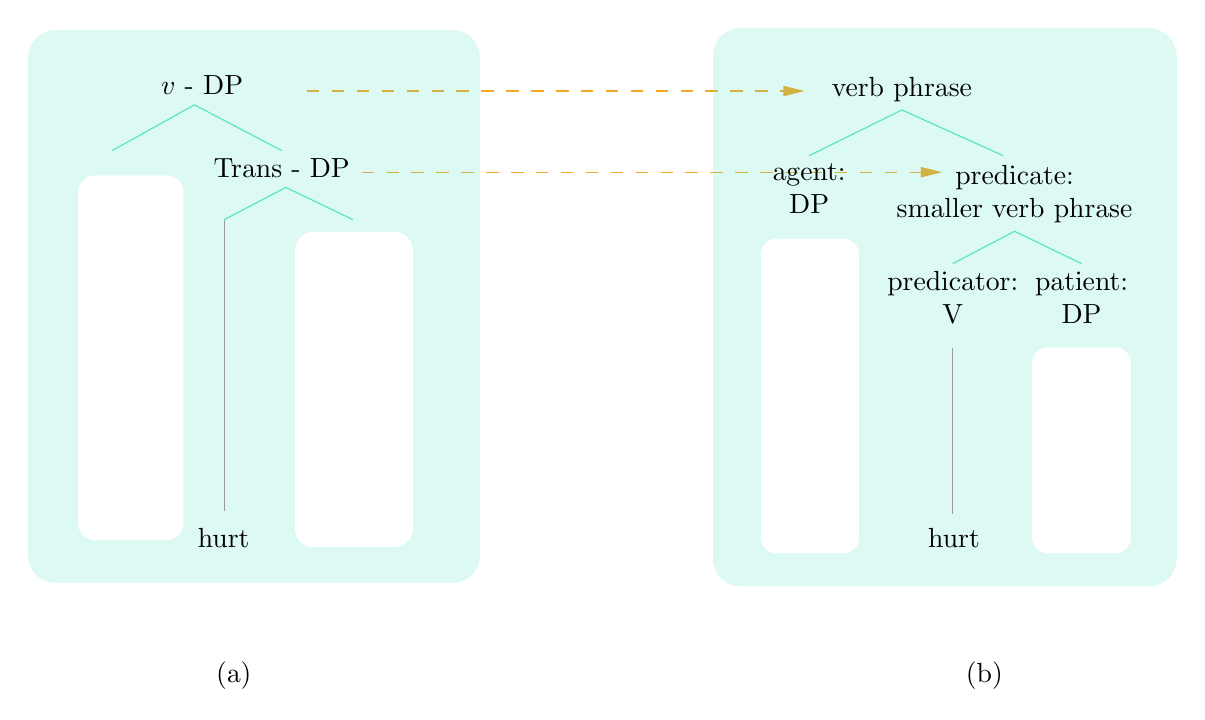
\begin{tikzpicture}[x=0.75pt,y=0.75pt,yscale=-0.85,xscale=0.85]
%uncomment if require: \path (0,408); %set diagram left start at 0, and has height of 408

%Straight Lines [id:da2665478368972569] 
\draw [color={rgb, 255:red, 245; green, 166; blue, 35 }  ,draw opacity=1 ] [dash pattern={on 4.5pt off 4.5pt}]  (264,61) -- (544,61) ;
\draw [shift={(546,61)}, rotate = 180] [fill={rgb, 255:red, 245; green, 166; blue, 35 }  ,fill opacity=1 ][line width=0.08]  [draw opacity=0] (12,-3) -- (0,0) -- (12,3) -- cycle    ;
%Straight Lines [id:da6278442099042232] 
\draw [color={rgb, 255:red, 245; green, 166; blue, 35 }  ,draw opacity=1 ] [dash pattern={on 4.5pt off 4.5pt}]  (295,107) -- (622,107) ;
\draw [shift={(624,107)}, rotate = 180] [fill={rgb, 255:red, 245; green, 166; blue, 35 }  ,fill opacity=1 ][line width=0.08]  [draw opacity=0] (12,-3) -- (0,0) -- (12,3) -- cycle    ;
%Rounded Rect [id:dp9005470977487176] 
\draw  [draw opacity=0][fill={rgb, 255:red, 80; green, 227; blue, 194 }  ,fill opacity=0.2 ] (494,41.22) .. controls (494,32.48) and (501.08,25.4) .. (509.82,25.4) -- (741.18,25.4) .. controls (749.92,25.4) and (757,32.48) .. (757,41.22) -- (757,325.99) .. controls (757,334.73) and (749.92,341.81) .. (741.18,341.81) -- (509.82,341.81) .. controls (501.08,341.81) and (494,334.73) .. (494,325.99) -- cycle ;
%Straight Lines [id:da3555404365615693] 
\draw [color={rgb, 255:red, 155; green, 155; blue, 155 }  ,draw opacity=1 ]   (630.05,206.81) -- (630.05,301) ;
%Straight Lines [id:da5116688308518689] 
\draw [color={rgb, 255:red, 80; green, 227; blue, 194 }  ,draw opacity=1 ]   (703.05,158.83) -- (665.05,140.5) ;
%Straight Lines [id:da7532901881200198] 
\draw [color={rgb, 255:red, 80; green, 227; blue, 194 }  ,draw opacity=1 ]   (665.05,140.5) -- (630.05,158.83) ;
%Straight Lines [id:da3708728686228633] 
\draw [color={rgb, 255:red, 80; green, 227; blue, 194 }  ,draw opacity=1 ]   (658.65,97.63) -- (601.2,71.73) ;
%Straight Lines [id:da18650265857430104] 
\draw [color={rgb, 255:red, 80; green, 227; blue, 194 }  ,draw opacity=1 ]   (601.2,71.73) -- (548.65,97.63) ;
%Rounded Rect [id:dp9951745940140804] 
\draw  [draw opacity=0][fill={rgb, 255:red, 255; green, 255; blue, 255 }  ,fill opacity=1 ] (675,215.16) .. controls (675,210.29) and (678.95,206.33) .. (683.83,206.33) -- (722.17,206.33) .. controls (727.05,206.33) and (731,210.29) .. (731,215.16) -- (731,314.17) .. controls (731,319.05) and (727.05,323) .. (722.17,323) -- (683.83,323) .. controls (678.95,323) and (675,319.05) .. (675,314.17) -- cycle ;
%Rounded Rect [id:dp4970986462373306] 
\draw  [draw opacity=0][fill={rgb, 255:red, 255; green, 255; blue, 255 }  ,fill opacity=1 ] (521.24,153.76) .. controls (521.24,148.82) and (525.25,144.81) .. (530.19,144.81) -- (568.05,144.81) .. controls (572.99,144.81) and (577,148.82) .. (577,153.76) -- (577,314.05) .. controls (577,318.99) and (572.99,323) .. (568.05,323) -- (530.19,323) .. controls (525.25,323) and (521.24,318.99) .. (521.24,314.05) -- cycle ;
%Rounded Rect [id:dp4071663798075751] 
\draw  [draw opacity=0][fill={rgb, 255:red, 80; green, 227; blue, 194 }  ,fill opacity=0.2 ] (106,41.89) .. controls (106,33.39) and (112.89,26.5) .. (121.4,26.5) -- (346.6,26.5) .. controls (355.11,26.5) and (362,33.39) .. (362,41.89) -- (362,324.41) .. controls (362,332.92) and (355.11,339.81) .. (346.6,339.81) -- (121.4,339.81) .. controls (112.89,339.81) and (106,332.92) .. (106,324.41) -- cycle ;
%Straight Lines [id:da5088138181155522] 
\draw [color={rgb, 255:red, 155; green, 155; blue, 155 }  ,draw opacity=1 ]   (217.05,133.93) -- (217.05,299.1) ;
%Straight Lines [id:da998446713157706] 
\draw [color={rgb, 255:red, 80; green, 227; blue, 194 }  ,draw opacity=1 ]   (290.05,133.93) -- (252.05,115.6) ;
%Straight Lines [id:da5752866187220778] 
\draw [color={rgb, 255:red, 80; green, 227; blue, 194 }  ,draw opacity=1 ]   (252.05,115.6) -- (217.05,133.93) ;
%Straight Lines [id:da6021628337779128] 
\draw [color={rgb, 255:red, 80; green, 227; blue, 194 }  ,draw opacity=1 ]   (249.65,94.73) -- (200.2,68.83) ;
%Straight Lines [id:da8361003247119008] 
\draw [color={rgb, 255:red, 80; green, 227; blue, 194 }  ,draw opacity=1 ]   (200.2,68.83) -- (153.65,94.73) ;
%Rounded Rect [id:dp3858870486231194] 
\draw  [draw opacity=0][fill={rgb, 255:red, 255; green, 255; blue, 255 }  ,fill opacity=1 ] (257.24,151.34) .. controls (257.24,145.52) and (261.96,140.81) .. (267.77,140.81) -- (313.48,140.81) .. controls (319.29,140.81) and (324,145.52) .. (324,151.34) -- (324,309.05) .. controls (324,314.86) and (319.29,319.57) .. (313.48,319.57) -- (267.77,319.57) .. controls (261.96,319.57) and (257.24,314.86) .. (257.24,309.05) -- cycle ;
%Rounded Rect [id:dp2951833006567197] 
\draw  [draw opacity=0][fill={rgb, 255:red, 255; green, 255; blue, 255 }  ,fill opacity=1 ] (134.24,118.4) .. controls (134.24,113.11) and (138.54,108.81) .. (143.84,108.81) -- (184.41,108.81) .. controls (189.71,108.81) and (194,113.11) .. (194,118.4) -- (194,305.98) .. controls (194,311.28) and (189.71,315.57) .. (184.41,315.57) -- (143.84,315.57) .. controls (138.54,315.57) and (134.24,311.28) .. (134.24,305.98) -- cycle ;

% Text Node
\draw (630.76,321) node [anchor=south] [inner sep=0.75pt]   [align=left] {hurt};
% Text Node
\draw (665.05,137.5) node [anchor=south] [inner sep=0.75pt]   [align=left] {\begin{minipage}[lt]{89.53pt}\setlength\topsep{0pt}
\begin{center}
predicate:\\smaller verb phrase
\end{center}

\end{minipage}};
% Text Node
\draw (601.2,68.73) node [anchor=south] [inner sep=0.75pt]   [align=left] {verb phrase};
% Text Node
\draw (548.65,100.63) node [anchor=north] [inner sep=0.75pt]   [align=left] {\begin{minipage}[lt]{29.61pt}\setlength\topsep{0pt}
\begin{center}
agent:\\DP
\end{center}

\end{minipage}};
% Text Node
\draw (630.05,161.83) node [anchor=north] [inner sep=0.75pt]   [align=left] {\begin{minipage}[lt]{50.89pt}\setlength\topsep{0pt}
\begin{center}
predicator:\\V
\end{center}

\end{minipage}};
% Text Node
\draw (703.05,161.83) node [anchor=north] [inner sep=0.75pt]   [align=left] {\begin{minipage}[lt]{36.95pt}\setlength\topsep{0pt}
\begin{center}
patient:\\DP
\end{center}

\end{minipage}};
% Text Node
\draw (216.76,321.1) node [anchor=south] [inner sep=0.75pt]   [align=left] {hurt};
% Text Node
\draw (249.65,97.73) node [anchor=north] [inner sep=0.75pt]   [align=left] {Trans - DP};
% Text Node
\draw (179.8,50.81) node [anchor=north west][inner sep=0.75pt]   [align=left] {$\displaystyle v$ - DP};
% Text Node
\draw (211,383) node [anchor=north west][inner sep=0.75pt]   [align=left] {(a)};
% Text Node
\draw (636,383) node [anchor=north west][inner sep=0.75pt]   [align=left] {(b)};


\end{tikzpicture}


    \caption{Routinized DM $v$P of the verb \emph{hurt}, with functional heads removed and the grammatical relations reserved}
    \label{fig:hurt-constituent-tree}
\end{figure}

The fact that derivational trees can be effectively routinized into pre-compiled trees 
raises the question about whether Minimalism is \emph{needed} at all.
Indeed, the framework used in \ac{cgel} is context-free \citep{pullum2008expressive}, 
and even after including the whole expressive power of Minimalism, 
what we get is just a mildly context sensitive grammar, or to be precise, 
a multiple context-free grammar \citep{clark2014introduction}.
Both CFGs and MCFGs are close to Standard Theory without movements, 
or to be frank, \emph{formalized American structuralist grammars},
and the necessity of all the fuss around Merge and its constraints is then questioned.
What is even worse for Minimalism is that certain types of CFGs and MCFGs 
seem to be easily learned via a quite domain-general learning algorithm,
and thus Minimalism may just be a good descriptive tool:
it shows the tendency of the human statistical learner,
but there is no domain-specific language faculty 
which is said to be described by Minimalism.
What we have in this circumstance is therefore a construction grammar with Minimalism flavor.

Note, however, that a typical Minimalist grammar is often mapped to a rather large MCFG, 
because of the expansion of all possible movements, feature configuration, etc. 
The fact that human languages are easier to describe in the Minimalist lens 
and not the strictly no-feature-no-movement MCFG lens may hint something about the human language faculty.
Even the actual case of human linguistic capacity is Minimalism-inspired construction grammar, 
the Minimalist flavor will still be very strong,
and what today's generative linguists do is still useful, 
even though their story about human language faculty needs adaption.

The routinized (and quite \ac{cgel}-like) constituency grammar formalism, 
especially after accompanied by the notion of complements and modifiers (\prettyref{sec:sub-cat}), 
is like the good old X-bar theory, where a lexical word 
(not a functional word, especially not an invisible functional head) heads a constituent 
with multiple complements, specifiers and adjuncts (all in generative terms). 
The main differences between the GB-like X-bar scheme and the \ac{cgel} scheme are 
that in the former terms like ``complement'' is defined strictly in structural terms 
(e.g. ``the sister of the head''), 
while in the latter these terms are defined in terms of dependency relations 
(e.g. ``complements are more explicitly licensed by the head than modifiers'') 
without any guarantee that complements are necessarily lower than modifiers \citep{payne2007fusion},
and that in the \ac{cgel} framework there is no intermediate projections: 
nominals in \ac{cgel} corresponds to N' projections in X-bar theory, 
but the former can appear as a complete unit (e.g. as the modifier of another NP). 

We can summarize that the framework in \ac{cgel} is a little more flexible than X-bar theory. 
From the Minimalism perspective, it is easy to explain why: 
the criteria \ac{cgel} uses to draw the line between complements and modifiers are related 
more to subcagegorization information that is shown in the fine-grained Minimalist tree 
but not the coarse-grained \ac{cgel} tree (\prettyref{sec:sub-cat}) 
and hints nothing about whether a constituent is a maximal projection or not. 
Purely tree structure-based notion of ``complements'' 
based on coarse-grained GB or \ac{cgel} trees 
is bond to fail. 
It is possible to define \term{complement} purely in terms of tree structure in Minimalism,
because all functional projections are present, 
and thus we can say, for example, 
that ``the specifier of the Trans projection is the O argument, etc. 
and A and O arguments are complements of a transitive verb'',
but in coarse-grained formalisms, 
these functional projections are blurred as in \prettyref{fig:hurt-constituent-tree}.
So-called intermediate projections in X-bar theory, like N', 
are actually maximal projections according to more fine-grained analysis, 
and hence they indeed can appear as a complete constituency in some occasions.

Another feature of the framework in \ac{cgel} that is more flexible than the old-fashioned
is that it displays the segmentation of different functional layers of an XP,
with X being a lexical head, 
while the old-fashioned X-bar theory does not shows the fine structure of the dependents 
between the lexical head and the specifier.
This is illustrated in \ac{cgel} \citesec{5.2} [11]:
the dependents introduced with a \emph{nominal} parent node 
belong to an inner functional domain, 
while dependents introduced with a \emph{NP} parent node 
belong to an external functional domain.
The functional domains catch the essential intuition of ``maximal projection'' in the X-bar scheme,
but if we are to implement the idea of two functional domains in terms of X-bar theory,
an asymmetry occurs: 
the lexical head (here it is the noun \term{salary}) cannot be the head of both the nominal and the NP,
so we have to find something else -- say the determiner -- as the head of the maximal projection 
corresponding to the external functional domain, and now we have both a lexical head and a functional head,
while the ways dependents are related to the lexical head and the functional head are different,
so the two heads are not ``heads'' in the same sense.
There are only two roads forward: 
one is to give up the idea of lexical heads altogether and use functional heads,
which leads to Minimalism,
while the other is to keep the notion of the lexical head 
but allow fine-grained segmentation of functional domains surrounding the head,
which leads to the \ac{cgel} -- and essentially \ac{blt} -- approach,
which is dual to the Minimalism approach (\prettyref{fig:cgel-minimalism-dual}).

\begin{figure}
    \centering
    

\tikzset{every picture/.style={line width=0.3pt}} %set default line width to 0.75pt        

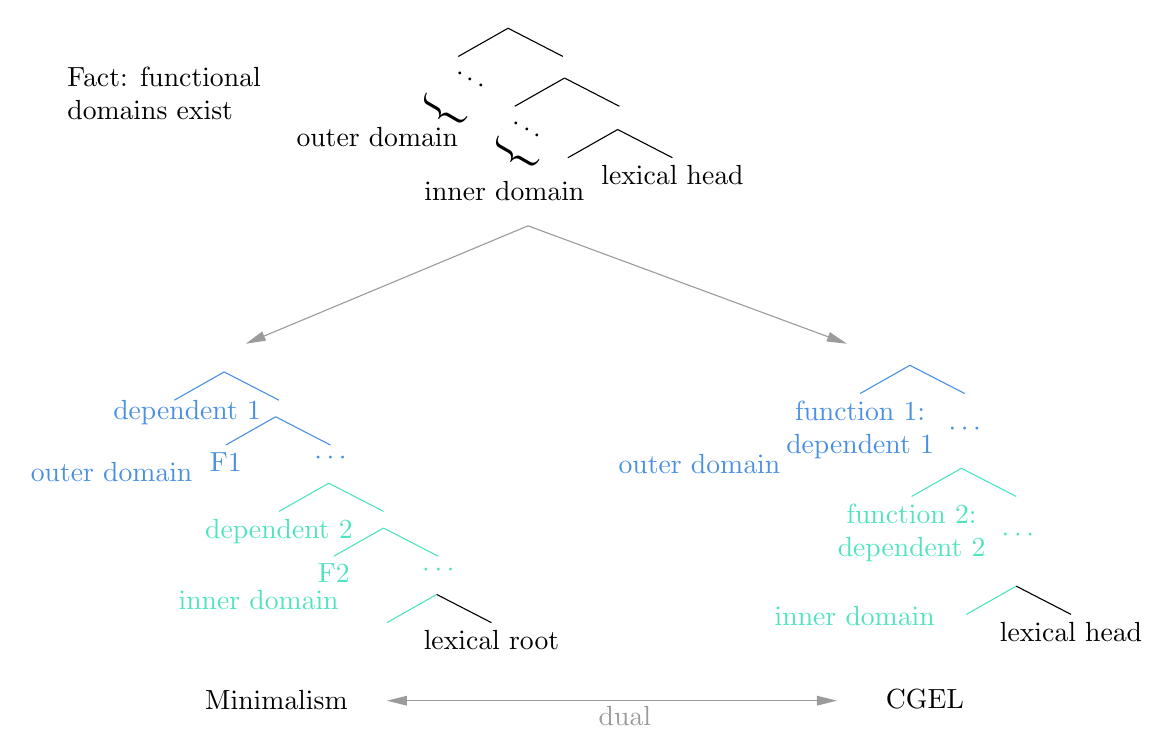
\begin{tikzpicture}[x=0.75pt,y=0.75pt,yscale=-0.8,xscale=0.8]
%uncomment if require: \path (0,523); %set diagram left start at 0, and has height of 523

%Straight Lines [id:da6705457534949089] 
\draw    (313,92.15) -- (343,75.15) ;
%Straight Lines [id:da28013820417559354] 
\draw    (376,92.15) -- (343,75.15) ;
%Straight Lines [id:da26185532929398736] 
\draw    (345,123.15) -- (375,106.15) ;
%Straight Lines [id:da1670225517468129] 
\draw    (408,123.15) -- (375,106.15) ;
%Straight Lines [id:da7951370858439135] 
\draw    (279,62.15) -- (309,45.15) ;
%Straight Lines [id:da5307564248915579] 
\draw    (342,62.15) -- (309,45.15) ;
%Straight Lines [id:da6264444449679678] 
\draw [color={rgb, 255:red, 155; green, 155; blue, 155 }  ,draw opacity=1 ]   (321,164.15) -- (152.85,234.38) ;
\draw [shift={(151,235.15)}, rotate = 337.33] [fill={rgb, 255:red, 155; green, 155; blue, 155 }  ,fill opacity=1 ][line width=0.08]  [draw opacity=0] (12,-3) -- (0,0) -- (12,3) -- cycle    ;
%Straight Lines [id:da99450357998767] 
\draw [color={rgb, 255:red, 80; green, 227; blue, 194 }  ,draw opacity=1 ]   (204,363.15) -- (234,346.15) ;
%Straight Lines [id:da7516847541397156] 
\draw [color={rgb, 255:red, 80; green, 227; blue, 194 }  ,draw opacity=1 ]   (267,363.15) -- (234,346.15) ;
%Straight Lines [id:da7086721116542554] 
\draw [color={rgb, 255:red, 80; green, 227; blue, 194 }  ,draw opacity=1 ]   (236,403.15) -- (266,386.15) ;
%Straight Lines [id:da23963037522787767] 
\draw    (299,403.15) -- (266,386.15) ;
%Straight Lines [id:da8629804052760564] 
\draw [color={rgb, 255:red, 74; green, 144; blue, 226 }  ,draw opacity=1 ]   (139,296.15) -- (146.67,291.8) -- (169,279.15) ;
%Straight Lines [id:da21212301774701436] 
\draw [color={rgb, 255:red, 74; green, 144; blue, 226 }  ,draw opacity=1 ]   (202,296.15) -- (169,279.15) ;
%Straight Lines [id:da45399705070135465] 
\draw [color={rgb, 255:red, 155; green, 155; blue, 155 }  ,draw opacity=1 ]   (321,164.15) -- (511.12,234.45) ;
\draw [shift={(513,235.15)}, rotate = 200.29] [fill={rgb, 255:red, 155; green, 155; blue, 155 }  ,fill opacity=1 ][line width=0.08]  [draw opacity=0] (12,-3) -- (0,0) -- (12,3) -- cycle    ;
%Straight Lines [id:da06579349148912339] 
\draw [color={rgb, 255:red, 80; green, 227; blue, 194 }  ,draw opacity=1 ]   (552,327.15) -- (582,310.15) ;
%Straight Lines [id:da7813158499201878] 
\draw [color={rgb, 255:red, 80; green, 227; blue, 194 }  ,draw opacity=1 ]   (615,327.15) -- (582,310.15) ;
%Straight Lines [id:da6554597016072419] 
\draw [color={rgb, 255:red, 80; green, 227; blue, 194 }  ,draw opacity=1 ]   (585,398.15) -- (615,381.15) ;
%Straight Lines [id:da38771820652223643] 
\draw    (648,398.15) -- (615,381.15) ;
%Straight Lines [id:da7029269298051468] 
\draw [color={rgb, 255:red, 74; green, 144; blue, 226 }  ,draw opacity=1 ]   (521,265.15) -- (528.67,260.8) -- (551,248.15) ;
%Straight Lines [id:da3078830979711833] 
\draw [color={rgb, 255:red, 74; green, 144; blue, 226 }  ,draw opacity=1 ]   (584,265.15) -- (551,248.15) ;
%Straight Lines [id:da5015548112989887] 
\draw [color={rgb, 255:red, 80; green, 227; blue, 194 }  ,draw opacity=1 ]   (171,336.15) -- (201,319.15) ;
%Straight Lines [id:da5954251542916287] 
\draw [color={rgb, 255:red, 80; green, 227; blue, 194 }  ,draw opacity=1 ]   (234,336.15) -- (201,319.15) ;
%Straight Lines [id:da4688878650352748] 
\draw [color={rgb, 255:red, 74; green, 144; blue, 226 }  ,draw opacity=1 ]   (108,269.15) -- (115.67,264.8) -- (138,252.15) ;
%Straight Lines [id:da2607503270176317] 
\draw [color={rgb, 255:red, 74; green, 144; blue, 226 }  ,draw opacity=1 ]   (171,269.15) -- (138,252.15) ;
%Straight Lines [id:da8702130416826466] 
\draw [color={rgb, 255:red, 155; green, 155; blue, 155 }  ,draw opacity=1 ]   (238,450.15) -- (505,450.15) ;
\draw [shift={(507,450.15)}, rotate = 180] [fill={rgb, 255:red, 155; green, 155; blue, 155 }  ,fill opacity=1 ][line width=0.08]  [draw opacity=0] (12,-3) -- (0,0) -- (12,3) -- cycle    ;
\draw [shift={(236,450.15)}, rotate = 0] [fill={rgb, 255:red, 155; green, 155; blue, 155 }  ,fill opacity=1 ][line width=0.08]  [draw opacity=0] (12,-3) -- (0,0) -- (12,3) -- cycle    ;

% Text Node
\draw (313.03,96.09) node [anchor=north west][inner sep=0.75pt]  [rotate=-30]  {$\cdots $};
% Text Node
\draw (408,126.15) node [anchor=north] [inner sep=0.75pt]   [align=left] {lexical head};
% Text Node
\draw (279.03,66.09) node [anchor=north west][inner sep=0.75pt]  [rotate=-30]  {$\cdots $};
% Text Node
\draw (42,67) node [anchor=north west][inner sep=0.75pt]   [align=left] {Fact: functional \\domains exist};
% Text Node
\draw (251.89,95.5) node [anchor=north west][inner sep=0.75pt]  [rotate=-300] [align=left] {{\LARGE \{}};
% Text Node
\draw (294.89,121.5) node [anchor=north west][inner sep=0.75pt]  [rotate=-300] [align=left] {{\LARGE \{}};
% Text Node
\draw (180,103) node [anchor=north west][inner sep=0.75pt]   [align=left] {outer domain};
% Text Node
\draw (257,136) node [anchor=north west][inner sep=0.75pt]   [align=left] {inner domain};
% Text Node
\draw (299,406.15) node [anchor=north] [inner sep=0.75pt]   [align=left] {lexical root};
% Text Node
\draw (20,305) node [anchor=north west][inner sep=0.75pt]  [color={rgb, 255:red, 74; green, 144; blue, 226 }  ,opacity=1 ] [align=left] {outer domain};
% Text Node
\draw (109,382) node [anchor=north west][inner sep=0.75pt]  [color={rgb, 255:red, 80; green, 227; blue, 194 }  ,opacity=1 ] [align=left] {inner domain};
% Text Node
\draw (139,299.15) node [anchor=north] [inner sep=0.75pt]  [color={rgb, 255:red, 74; green, 144; blue, 226 }  ,opacity=1 ] [align=left] {F1};
% Text Node
\draw (204,366.15) node [anchor=north] [inner sep=0.75pt]  [color={rgb, 255:red, 80; green, 227; blue, 194 }  ,opacity=1 ] [align=left] {F2};
% Text Node
\draw (125,442.15) node [anchor=north west][inner sep=0.75pt]   [align=left] {Minimalism};
% Text Node
\draw (648,401.15) node [anchor=north] [inner sep=0.75pt]   [align=left] {lexical head};
% Text Node
\draw (374,300) node [anchor=north west][inner sep=0.75pt]  [color={rgb, 255:red, 74; green, 144; blue, 226 }  ,opacity=1 ] [align=left] {outer domain};
% Text Node
\draw (468,392) node [anchor=north west][inner sep=0.75pt]  [color={rgb, 255:red, 80; green, 227; blue, 194 }  ,opacity=1 ] [align=left] {inner domain};
% Text Node
\draw (521,268.15) node [anchor=north] [inner sep=0.75pt]  [color={rgb, 255:red, 74; green, 144; blue, 226 }  ,opacity=1 ] [align=left] {\begin{minipage}[lt]{57.07pt}\setlength\topsep{0pt}
\begin{center}
function 1:\\dependent 1\\
\end{center}

\end{minipage}};
% Text Node
\draw (552,330.15) node [anchor=north] [inner sep=0.75pt]  [color={rgb, 255:red, 80; green, 227; blue, 194 }  ,opacity=1 ] [align=left] {\begin{minipage}[lt]{57.07pt}\setlength\topsep{0pt}
\begin{center}
function 2:\\dependent 2
\end{center}

\end{minipage}};
% Text Node
\draw (171,339.15) node [anchor=north] [inner sep=0.75pt]  [color={rgb, 255:red, 80; green, 227; blue, 194 }  ,opacity=1 ] [align=left] {dependent 2};
% Text Node
\draw (115.67,267.8) node [anchor=north] [inner sep=0.75pt]  [color={rgb, 255:red, 74; green, 144; blue, 226 }  ,opacity=1 ] [align=left] {dependent 1};
% Text Node
\draw (202,299.15) node [anchor=north] [inner sep=0.75pt]  [color={rgb, 255:red, 74; green, 144; blue, 226 }  ,opacity=1 ] [align=left] {$\displaystyle \cdots $};
% Text Node
\draw (267,366.15) node [anchor=north] [inner sep=0.75pt]  [color={rgb, 255:red, 80; green, 227; blue, 194 }  ,opacity=1 ] [align=left] {$\displaystyle \cdots $};
% Text Node
\draw (584,281.15) node [anchor=north] [inner sep=0.75pt]  [color={rgb, 255:red, 74; green, 144; blue, 226 }  ,opacity=1 ] [align=left] {$\displaystyle \cdots $};
% Text Node
\draw (616,345.15) node [anchor=north] [inner sep=0.75pt]  [color={rgb, 255:red, 80; green, 227; blue, 194 }  ,opacity=1 ] [align=left] {$\displaystyle \cdots $};
% Text Node
\draw (535,442) node [anchor=north west][inner sep=0.75pt]   [align=left] {CGEL};
% Text Node
\draw (362,452.15) node [anchor=north west][inner sep=0.75pt]  [color={rgb, 255:red, 155; green, 155; blue, 155 }  ,opacity=1 ] [align=left] {dual};


\end{tikzpicture}

    \caption{Functional domains in \ac{cgel} and Minimalism}
    \label{fig:cgel-minimalism-dual}
\end{figure}

The X-bar theory is therefore just a transitional version of generative syntax 
between the more surface-oriented formalisms 
and the more fine-grained formalisms.

\subsubsection{Movements}\label{sec:movement-in-theory}

Whenever dependency relations that cannot be transparently reflected by a phrase structure grammar occur
(i.e. ill-nestedness occurs), movements occur \citep{boston2009dependency}. 
Let us consider the Spec-$v$P-to-Spec-TP A-movement of the subject in \prettyref{fig:coarse-grained-hurt-the-dog-badly}. We see the notion of this movement is just reflection of the fact 
that the subject both has an ``obligatory topic'' position (in the terms of typology) in the whole clause 
and an agent position in the argument structure. There are two dependency relations involving it, and 
the movement-free phrase structure grammar can only easily reflect one, and thus we need a movement 
if we want to show all dependency relations with constituency structure. Some formalisms, like HPSG,
reject the notion of movement, but introduce an ``agent'' feature in the feature structure of 
VP, which is merely movement in feature structure's disguise. 

\begin{figure}
    \centering
    

\tikzset{every picture/.style={line width=0.3pt}} %set default line width to 0.75pt        

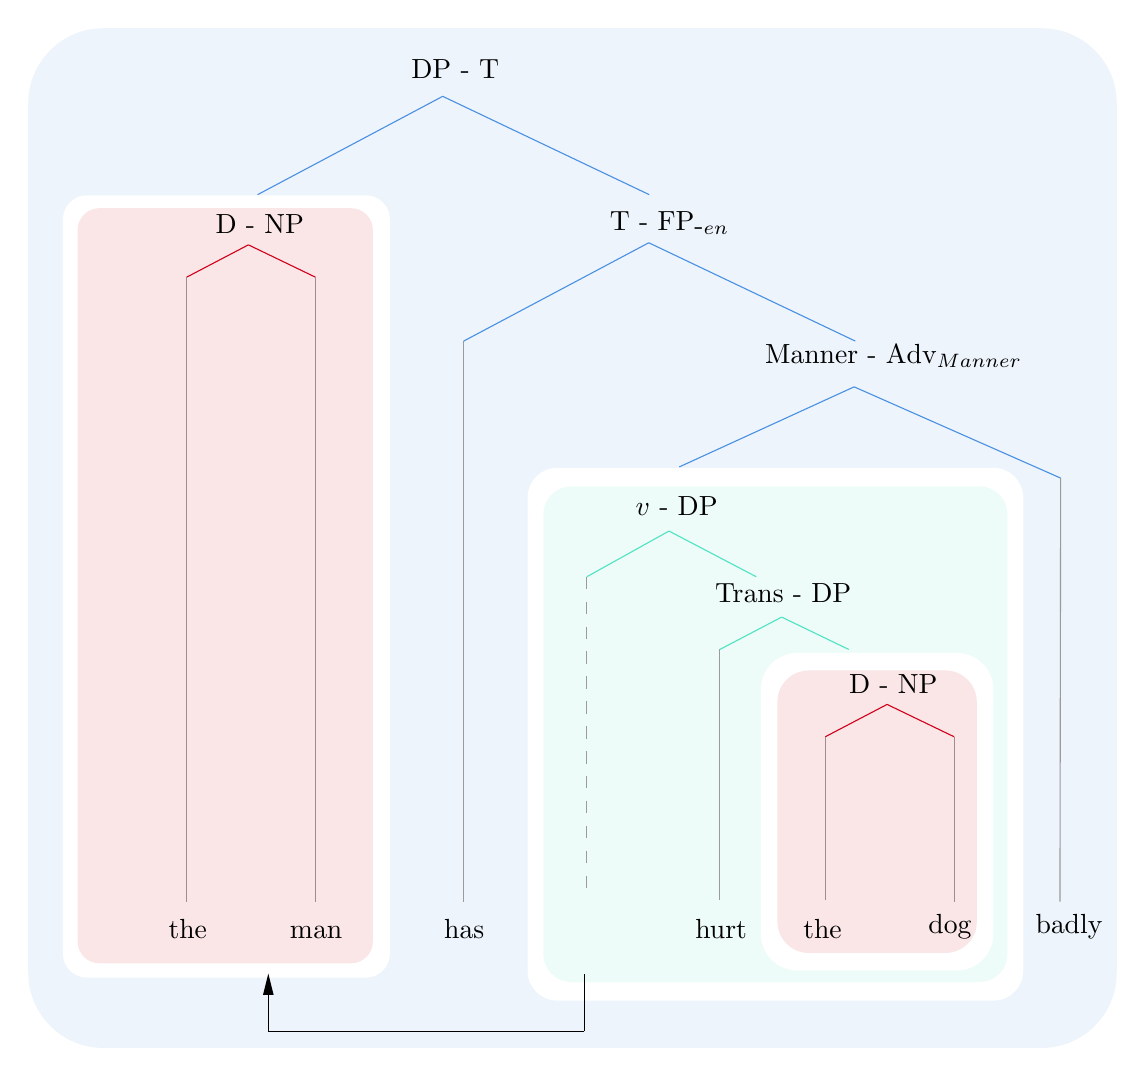
\begin{tikzpicture}[x=0.75pt,y=0.75pt,yscale=-0.85,xscale=0.85]
%uncomment if require: \path (0,709); %set diagram left start at 0, and has height of 709

%Rounded Rect [id:dp034885216520763374] 
\draw  [draw opacity=0][fill={rgb, 255:red, 74; green, 144; blue, 226 }  ,fill opacity=0.1 ] (88,80.93) .. controls (88,57.41) and (107.07,38.33) .. (130.6,38.33) -- (662.4,38.33) .. controls (685.93,38.33) and (705,57.41) .. (705,80.93) -- (705,573.73) .. controls (705,597.26) and (685.93,616.33) .. (662.4,616.33) -- (130.6,616.33) .. controls (107.07,616.33) and (88,597.26) .. (88,573.73) -- cycle ;
%Rounded Rect [id:dp864413197045051] 
\draw  [draw opacity=0][fill={rgb, 255:red, 255; green, 255; blue, 255 }  ,fill opacity=1 ] (371,304.4) .. controls (371,295.07) and (378.57,287.5) .. (387.9,287.5) -- (635.1,287.5) .. controls (644.43,287.5) and (652,295.07) .. (652,304.4) -- (652,572.6) .. controls (652,581.93) and (644.43,589.5) .. (635.1,589.5) -- (387.9,589.5) .. controls (378.57,589.5) and (371,581.93) .. (371,572.6) -- cycle ;
%Rounded Rect [id:dp31861860103211814] 
\draw  [draw opacity=0][fill={rgb, 255:red, 80; green, 227; blue, 194 }  ,fill opacity=0.1 ] (380,313.82) .. controls (380,305.08) and (387.08,298) .. (395.82,298) -- (627.18,298) .. controls (635.92,298) and (643,305.08) .. (643,313.82) -- (643,563.18) .. controls (643,571.92) and (635.92,579) .. (627.18,579) -- (395.82,579) .. controls (387.08,579) and (380,571.92) .. (380,563.18) -- cycle ;
%Rounded Rect [id:dp23576358575832845] 
\draw  [draw opacity=0][fill={rgb, 255:red, 255; green, 255; blue, 255 }  ,fill opacity=1 ] (503.24,413.2) .. controls (503.24,401.72) and (512.55,392.42) .. (524.03,392.42) -- (614.3,392.42) .. controls (625.78,392.42) and (635.08,401.72) .. (635.08,413.2) -- (635.08,551.63) .. controls (635.08,563.11) and (625.78,572.42) .. (614.3,572.42) -- (524.03,572.42) .. controls (512.55,572.42) and (503.24,563.11) .. (503.24,551.63) -- cycle ;
%Rounded Rect [id:dp7324546519566175] 
\draw  [draw opacity=0][fill={rgb, 255:red, 255; green, 255; blue, 255 }  ,fill opacity=1 ] (107.67,146.66) .. controls (107.67,139.12) and (113.78,133) .. (121.33,133) -- (279.34,133) .. controls (286.88,133) and (293,139.12) .. (293,146.66) -- (293,562.84) .. controls (293,570.38) and (286.88,576.5) .. (279.34,576.5) -- (121.33,576.5) .. controls (113.78,576.5) and (107.67,570.38) .. (107.67,562.84) -- cycle ;
%Straight Lines [id:da3972557940014332] 
\draw [color={rgb, 255:red, 208; green, 2; blue, 27 }  ,draw opacity=1 ]   (250.8,179.44) -- (212.8,161.11) ;
%Straight Lines [id:da3734280152933176] 
\draw [color={rgb, 255:red, 208; green, 2; blue, 27 }  ,draw opacity=1 ]   (212.8,161.11) -- (177.8,179.44) ;
%Straight Lines [id:da8957091119411691] 
\draw [color={rgb, 255:red, 208; green, 2; blue, 27 }  ,draw opacity=1 ]   (612.8,439.93) -- (574.8,421.6) ;
%Straight Lines [id:da8730392291245619] 
\draw [color={rgb, 255:red, 208; green, 2; blue, 27 }  ,draw opacity=1 ]   (574.8,421.6) -- (539.8,439.93) ;
%Straight Lines [id:da36657403374376774] 
\draw [color={rgb, 255:red, 155; green, 155; blue, 155 }  ,draw opacity=1 ]   (539.8,439.93) -- (539.8,532.6) ;
%Straight Lines [id:da11962397518947854] 
\draw [color={rgb, 255:red, 155; green, 155; blue, 155 }  ,draw opacity=1 ]   (612.8,439.93) -- (612.8,533.4) ;
%Straight Lines [id:da4999235058666789] 
\draw [color={rgb, 255:red, 155; green, 155; blue, 155 }  ,draw opacity=1 ]   (480.05,390.43) -- (480.05,532.6) ;
%Straight Lines [id:da6548410354329881] 
\draw [color={rgb, 255:red, 80; green, 227; blue, 194 }  ,draw opacity=1 ]   (553.05,390.43) -- (515.05,372.1) ;
%Straight Lines [id:da2235852996451071] 
\draw [color={rgb, 255:red, 80; green, 227; blue, 194 }  ,draw opacity=1 ]   (515.05,372.1) -- (480.05,390.43) ;
%Straight Lines [id:da0769185876775682] 
\draw [color={rgb, 255:red, 80; green, 227; blue, 194 }  ,draw opacity=1 ]   (500.65,349.23) -- (451.2,323.33) ;
%Straight Lines [id:da7127264168717515] 
\draw [color={rgb, 255:red, 80; green, 227; blue, 194 }  ,draw opacity=1 ]   (451.2,323.33) -- (404.65,349.23) ;
%Straight Lines [id:da1867123098813408] 
\draw [color={rgb, 255:red, 155; green, 155; blue, 155 }  ,draw opacity=1 ] [dash pattern={on 4.5pt off 4.5pt}]  (404.65,349.23) -- (404.65,532.5) ;
%Straight Lines [id:da4924213637331023] 
\draw [color={rgb, 255:red, 74; green, 144; blue, 226 }  ,draw opacity=1 ]   (673.2,293.33) -- (556.13,241.6) ;
%Straight Lines [id:da3715548654487917] 
\draw [color={rgb, 255:red, 74; green, 144; blue, 226 }  ,draw opacity=1 ]   (556.13,241.6) -- (457,287) ;
%Straight Lines [id:da022458887362470925] 
\draw [color={rgb, 255:red, 155; green, 155; blue, 155 }  ,draw opacity=1 ]   (673.2,293.33) -- (672.8,533.4) ;
%Straight Lines [id:da084129560695545] 
\draw [color={rgb, 255:red, 155; green, 155; blue, 155 }  ,draw opacity=1 ]   (334.8,215.67) -- (334.8,533.4) ;
%Straight Lines [id:da11283861445316812] 
\draw [color={rgb, 255:red, 74; green, 144; blue, 226 }  ,draw opacity=1 ]   (556.8,215.67) -- (439.73,159.93) ;
%Straight Lines [id:da18405698017218852] 
\draw [color={rgb, 255:red, 74; green, 144; blue, 226 }  ,draw opacity=1 ]   (439.73,159.93) -- (334.8,215.67) ;
%Straight Lines [id:da4142916860805901] 
\draw [color={rgb, 255:red, 155; green, 155; blue, 155 }  ,draw opacity=1 ]   (250.8,179.44) -- (250.8,533.4) ;
%Straight Lines [id:da9820239195731701] 
\draw [color={rgb, 255:red, 155; green, 155; blue, 155 }  ,draw opacity=1 ]   (177.8,179.44) -- (177.8,533.4) ;
%Straight Lines [id:da8912900354325306] 
\draw [color={rgb, 255:red, 74; green, 144; blue, 226 }  ,draw opacity=1 ]   (440,132.67) -- (322.93,76.93) ;
%Straight Lines [id:da46428872338489646] 
\draw [color={rgb, 255:red, 74; green, 144; blue, 226 }  ,draw opacity=1 ]   (322.93,76.93) -- (218,132.67) ;
%Straight Lines [id:da27398889935539716] 
\draw    (403.27,606.8) -- (224.07,606.8) ;
%Straight Lines [id:da6293499120506956] 
\draw    (403.27,606.8) -- (403.27,574.2) ;
%Straight Lines [id:da1448979089622664] 
\draw    (224.07,606.8) -- (224.07,576.2) ;
\draw [shift={(224.07,574.2)}, rotate = 90] [fill={rgb, 255:red, 0; green, 0; blue, 0 }  ][line width=0.08]  [draw opacity=0] (12,-3) -- (0,0) -- (12,3) -- cycle    ;
%Rounded Rect [id:dp49028218668622503] 
\draw  [draw opacity=0][fill={rgb, 255:red, 208; green, 2; blue, 27 }  ,fill opacity=0.1 ] (116,152.67) .. controls (116,145.86) and (121.52,140.33) .. (128.33,140.33) -- (271,140.33) .. controls (277.81,140.33) and (283.33,145.86) .. (283.33,152.67) -- (283.33,556) .. controls (283.33,562.81) and (277.81,568.33) .. (271,568.33) -- (128.33,568.33) .. controls (121.52,568.33) and (116,562.81) .. (116,556) -- cycle ;
%Rounded Rect [id:dp8649953827045236] 
\draw  [draw opacity=0][fill={rgb, 255:red, 208; green, 2; blue, 27 }  ,fill opacity=0.1 ] (512.66,420.15) .. controls (512.66,410.31) and (520.64,402.33) .. (530.47,402.33) -- (607.85,402.33) .. controls (617.69,402.33) and (625.67,410.31) .. (625.67,420.15) -- (625.67,544.69) .. controls (625.67,554.52) and (617.69,562.5) .. (607.85,562.5) -- (530.47,562.5) .. controls (520.64,562.5) and (512.66,554.52) .. (512.66,544.69) -- cycle ;

% Text Node
\draw (178.41,556) node [anchor=south] [inner sep=0.75pt]   [align=left] {the};
% Text Node
\draw (251.16,556) node [anchor=south] [inner sep=0.75pt]   [align=left] {man};
% Text Node
\draw (335.07,556) node [anchor=south] [inner sep=0.75pt]   [align=left] {has};
% Text Node
\draw (480.76,556) node [anchor=south] [inner sep=0.75pt]   [align=left] {hurt};
% Text Node
\draw (538.21,556) node [anchor=south] [inner sep=0.75pt]   [align=left] {the};
% Text Node
\draw (610.47,556) node [anchor=south] [inner sep=0.75pt]   [align=left] {dog};
% Text Node
\draw (677.91,556) node [anchor=south] [inner sep=0.75pt]   [align=left] {badly};
% Text Node
\draw (551.8,403.27) node [anchor=north west][inner sep=0.75pt]   [align=left] {D - NP};
% Text Node
\draw (475.8,351.52) node [anchor=north west][inner sep=0.75pt]   [align=left] {Trans - DP};
% Text Node
\draw (430.8,302.32) node [anchor=north west][inner sep=0.75pt]   [align=left] {$\displaystyle v$ - DP};
% Text Node
\draw (504.2,216) node [anchor=north west][inner sep=0.75pt]   [align=left] {Manner - Adv$\displaystyle _{\text{Manner}}$};
% Text Node
\draw (416.2,140.8) node [anchor=north west][inner sep=0.75pt]   [align=left] {T - FP$\displaystyle _{\text{\mbox{-}en}}$};
% Text Node
\draw (192.67,142.44) node [anchor=north west][inner sep=0.75pt]   [align=left] {D - NP};
% Text Node
\draw (303.67,54.6) node [anchor=north west][inner sep=0.75pt]   [align=left] {DP - T};


\end{tikzpicture}

    \caption{The coarse-grained version of the Minimalist derivation of \emph{The man has hurt the dog badly}}
    \label{fig:coarse-grained-hurt-the-dog-badly}
\end{figure}

If the dual status of the subject is not reflected by movement or by feature structure, 
it either has to be reflected by something outside the tree, 
or has to be reflected by enumerating all possible construction types. 
It is easy to see that although surface-oriented grammarians are mostly more pragmatic than generative linguists, 
sticking to the surface form sometimes creates unnecessary burdens. 
Rejecting obligatory A-movements or equivalent notions totally means the linguist has to 
describe the TP structure and the argument structure always at the same time, 
which is tiresome both for the linguist and for the reader. 
But this does not mean A-movement appears in the name of \term{movement}, either:
enumerating all \emph{obligatory} grammatical categories in the TP
is still feasible,
and thus we can first describe a minimal canonical construction 
and then introduce adjunctions and transformations to non-canonical constructions.
% TODO: diagram

\subsubsection{Selection and subcagegorization, complements and modifiers}\label{sec:sub-cat}

\prettyref{fig:coarse-grained-hurt-the-dog-badly} contains an adverb, 
traditionally considered as an \emph{adjunct} in generative terms, 
which is optional and is largely invisible to multiple syntactic constraints. 
In the terms of \ac{cgel}, it is a \emph{modifier}, 
while \emph{the dog} and \emph{the man} are \emph{complements}.%
\footnote{\ac{cgel} uses the term ``adjunct'' for clausal modifiers.}
The main differences between complements and modifiers 
is that the former is licensed or even selected by the \ac{cgel} head of a constituent, 
which is also an important classification criterion 
of the lexical category of the head (known as \concept{subcategorization}),
while the latter can occur in a freer manner. 
In \ac{tag}, therefore, modifiers are introduced via adjunction, 
while complements are introduced via substitution.
This distinction has some theoretical backgrounds.
It may be assume that licensors of complements are essential for the spellout of the lexical head word
(which is the approach to subcagegorization in \citet{siddiqi2009syntax}).

Still, the distinction between complements and modifiers are opaque with 
the above argument about licensing and selection, 
and this opaqueness is again theoretically rooted. 
Languages with a relatively fixed word order often impose 
a word order constraints on clausal adjuncts and adjectives in NPs, 
which is well explained by the cartographic approach in which modifiers 
are introduced by a fixed hierarchy of functional heads. 
Tt follows that adjectives about different properties fill different ``slots of modifiers'' of the head noun, 
and similarly adjuncts about different properties fill different ``slots of modifiers'' of the head verb, 
in exactly the same way arguments fill argument slots in \prettyref{fig:hurt-constituent-tree}. 

Note that I say ``licensed \emph{or} even selected'' just before.
If a dependent has strong correlation with the head, it is a complement,
otherwise it is a modifier.
Logically, whether a dependent is required is independent of whether a dependent is a complement or a modifier.
The complement position may not be filled for some heads.
In English, for example, nouns take complements,
but these complements are rarely \emph{required} (\ac{cgel} \citesec{5.1.2}).
Obligatory dependents can be understood as generated in core projection layers,
while others can be understood as generated in optional projection layers \cite{pan2022deriving}.
This also justifies the \ac{tag} distinction between substitution and adjunction:
we may view the core projection layers as a prototypical and minimal example of the construction type in question,
and optional projection layers can be said to be adjoined into the minimal construction.
The existence of the adjunction operation means it is unnecessary
to routinize the whole Cinque hierarchy into something like \prettyref{fig:hurt-constituent-tree}.
Rather, we can first describe a minimal clause, 
and then go on to introduce possible optional dependents via adjunction. 
An obligatory dependent, however, is always considered as a complement, 
because if a dependent is obligatory, 
it is almost always the case that it has some close licensing relation with the lexical head,
though not all complements are obligatory.

Another remark here is that 
though complements are usually in lower positions in the phrase structure than modifiers,
this is not always the case.
\ac{cgel} \citesec{5.2} [11] is an example. 
If this analysis is considered controversial, 
then I have a definitely uncontroversial example: the subject.
If the $v$P layer and the TP layer are considered as forming a single construction (i.e. the nucleus clause),
and we ignore the inner Spec$v$P copy of the subject,
then the subject -- a complement -- is obviously on a higher position than the adjuncts, which are modifiers.
Whether a dependent is a complement or a modifier hints nothing about its syntactic position. 
What is -- and is not -- a complement is decided by the above listed tests, 
not by anything else.
And that is why in \ac{cgel}, though \emph{kindly} in \emph{He treats us kindly} is a complement,
it is, however, discussed together with clausal modifiers (or ``adjuncts'' in \ac{cgel} terms):
because \emph{kindly} is in the adverbial functional domain, anyway.
It makes sense to separate dependents in terms of functional domains:
this is how \ac{cgel} discusses clausal dependents, 
where \citechap{4} is about the prototypically ``complement'' domain,
but a kind of predicative -- which turns out to be adjunct -- 
is discussed in this chapter, 
and \citechap{8} is about prototypically ``adjunct'' or ``adverbial'' domain,
while manner complements, etc. are discussed in this chapter.

The conclusion that a clear distinction between complements and modifiers -- 
or in the case of clause structure, arguments and adjuncts -- 
is of limited purely formal interest and 
is better viewed as a language-specific descriptive concept \citep{haspelmath2014arguments}. 

\subsubsection{More discussion on dependents}\label{sec:dependents-types-enumerate}

Some dependents do not fit into the complement-modifier dichotomy, 
including the determiner, the classifier, etc.
Many of them are filled by functional words,
wile prototypical complements and modifiers are filled by lexical (phrasal) categories.
But there is no strict relation 
between being neither complement nor modifier 
and being filled functional words.
A determiner in English, for example, 
can be a genitive NP, 
so what fills a position that is neither complement nor modifier 
is not necessarily a functional word.
On the other hand, 
as is shown in \prettyref{chap:non-argument-complement},
certain types of non-argument complements have limited variation 
and it is reasonable to consider them as filled by functional words,
so functional words can fill complement positions. 

\subsubsection{Categories, heads and the notion of ``word''}

A \concept{category}\index{category} is defined as a type of constructions with similar distributions.
I will first discuss basic syntactic constructions and identify positions that can be filled in them, 
and then search possible constructions in these positions. This is how categories can be recognized.

A construction that is small enough is said to be a \concept{word} or more precisely, 
a \concept{grammatical word}\index{word!grammatical}.
I emphasize \emph{grammatical} because it is quite common to use the term \emph{word} 词 to denote 
a \concept{prosody word}\index{word!prosody}. Prosody is important in Chinese, which is discussed in 
\prettyref{sec:prosody-intro} and \prettyref{chap:prosody-overview}. 

In traditional grammars concerning Latin, 
a common practice is to roughly define word classes (nouns, verbs, etc.) 
according to their meaning and then discuss where they can be used. 
In this book I do not take this approach. 
Though I will review a lot of work based on the meaning-first approach, 
the way I distinguish word classes is mainly distributional. 
If two words can appear in similar positions, 
they are classified into one \concept{word class}\index{word class} or \concept{part of speech}.
A word class is just a category about words.  

In other words, I define concepts like \emph{noun-like} and \emph{verb-like} \emph{before} listing criteria of 
what is a noun and what is a verb. Criteria for word classes are always language-specific, but we have more 
confidence that at least some \emph{features} -- like the nominal feature \textit{n} or the verbal feature 
\textit{v} -- are cross-linguistic and may be attributed to the language faculty in the broad sense. 

\subsubsection{Dependency relations as in dependency grammars}\label{sec:dependency}



\subsubsection{Diverging standards of constituency revisited}

So now it is easy to see what is really going on in the flat trees in \ac{blt}: a constituent
is a large \emph{layer} in generative syntax, with grammatical relations inward being shown as 
dependency arcs instead of constituency hierarchy. 

\subsubsection{Empty categories and fusion-function constructions}

\subsubsection{Feature structures}


\section{Descriptive terms}\label{sec:descriptive-terms}

I have paid length discussions of \emph{structures} 
and demonstrated that the superfluously diverging frameworks are actually almost the same. 
But the formalism of generative syntax is probably not what dissatisfies field linguists the most.
Having worked out a \emph{formal} grammatical framework, 
a list of \emph{building blocks} are still required for fully describing a language. 
The former is purely about how structures are built, 
while the latter is about what raw materials are fed into the structure building machine. 
Universals about the former and the latter are called formal and substantial universals,respectively. 
Now readers of \ac{blt} will find 
what Dixon complains most about is not about the binary branching trees, 
but the tendency of ``formalists'' to find things equivalent to English in newly documented languages. 
In his depiction, formalists assume there are infinitives, 
inflection-derivation distinction, etc. in all languages, which he mocks several times. 
This depiction is actually not quite true for most generative works 
but is alarming for people seeking universal glossing and annotation rules.

What is discussed in this section is to find a set of grammatical relations 
as in \prettyref{fig:hurt-constituent-tree} (especially in (b), 
since most people in the descriptive community rejects 
all the functional hierarchies proposed in generative syntax).
This has already be done for English in \ac{cgel}. 
We already know some examples of these grammatical relations: 
\prettyref{sec:sub-cat}, for example, discusses complements and modifiers.
\ac{cgel} contains more grammatical relations: 
readers will find prenucleus positions in the clause, 
which are roughly specifier positions in the CP layer,
and also ``external modifiers'' in NPs. % TODO: 这些位置对应什么? 

\subsection{Clause structure}

\subsubsection{Predicate}

We use the term \concept{predicate} to denote the constituent containing the verb complex, 
complements that are not extracted out (most frequently, the object), some adverbials, etc.
This notion is problematic for the surface analysis of a VSO language, 
where head movement analysis is unavoidable, 
or otherwise clumsily enumerating all possible clause constructions 
(i.e. ``expanding the phrase structures'') is needed
but fortunately this is not the case in Chinese. 
The predicate is roughly TP minus the layer in which the subject is introduced. 
Note that the term \emph{predicate} is about syntactic function 
and has nothing to do with its inner structure.

A predicate, if with a lexical verb, is a \concept{verb phrase (VP)}.
The concept of VP is about syntactic form, not function. 
Though a cartographic grammarian may assume a $v$P in every clause, 
but it is then possible that the $v$ head is not realized on something that looks like a verb. 
It is, then, also possible that the predicate is not a typical VP.
This is indeed the case in some languages where a NP functions as the predicate \citep[\citesec{10.1.2}]{Friesen2017}.
\ac{blt} calls this ``verbless clause''.

\subsubsection{Complement in a clause, argument or not}\label{sec:complement-argument-clause}

It should also be noted that the term \emph{argument} is not the same as the term \concept{complement}, 
although the term \emph{argument-adjunct distinction} 
is much more frequent than the \ac{cgel}-style \emph{complement-modifier distinction}. 
In \ac{blt} terms, arguments include \emph{peripheral arguments},
like locative NPs or instrumental NPs, or even PPs 
(\ac{blt} insists that PPs are actually NPs with syntactic rather than morphological case markers), 
so some arguments are modifiers with the definition in \ac{cgel}. 
Even when we limit ourselves to core arguments, 
there is still a question whether all complements can be said to be arguments. 
Nominal complements are of course arguments, 
but complement clauses are less nominal 
since across languages they usually do not have person, number, gender and case 
(or so-called \concept{$\phi$-features} in generative terms). 
Some say it is still kind of nominal, 
and the complementizer is argued by some people to implicitly carry $\phi$-features \citep{complement-clause}.
Indeed, in traditional grammars, complement clauses are often named as ``nominal clauses''.

% TODO: more disucssion
The classification of clausal dependents in typical European languages is shown in \prettyref{fig:clause-dependent-classification}.

Telling arguments from the general notion of complements is important in Chinese grammar 
because in Chinese there are obviously non-argument particles which are licensed by the verb, 
commonly called 补语 ``complement'' in Chinese School Grammars (\prettyref{sec:school-grammar}).
Now there is a terminology confusion: we have two kinds of \ac{cgel} complements:
the first covers the arguments, and the second covers the non-argument complements, i.e. 补语 (\prettyref{chap:non-argument-complement}).
What makes things even more complicated is that certain so-called non-argument complements 
look like grammatical words, which have a finite number and can be enumerated (\prettyref{sec:complement-name}).
Therefore, in the Chinese version of \prettyref{fig:clause-dependent-classification},
we need a third axis about how close a constituent is to a grammatical word.

\begin{figure}
    \centering
    

\tikzset{every picture/.style={line width=0.75pt}} %set default line width to 0.75pt        

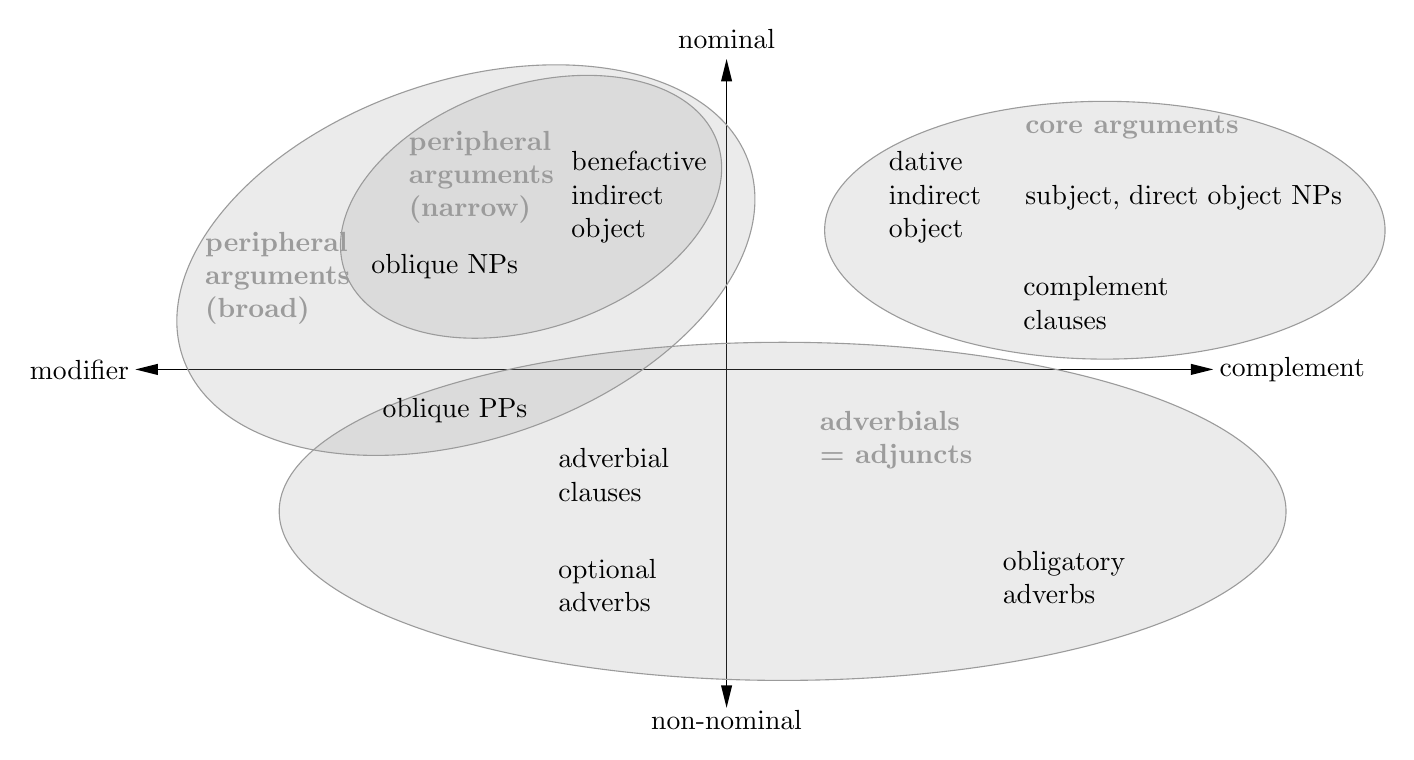
\begin{tikzpicture}[x=0.75pt,y=0.75pt,yscale=-0.9,xscale=0.9]
%uncomment if require: \path (0,401); %set diagram left start at 0, and has height of 401

%Straight Lines [id:da009476237276789146] 
\draw    (98,198) -- (671,198) ;
\draw [shift={(673,198)}, rotate = 180] [fill={rgb, 255:red, 0; green, 0; blue, 0 }  ][line width=0.08]  [draw opacity=0] (12,-3) -- (0,0) -- (12,3) -- cycle    ;
\draw [shift={(96,198)}, rotate = 0] [fill={rgb, 255:red, 0; green, 0; blue, 0 }  ][line width=0.08]  [draw opacity=0] (12,-3) -- (0,0) -- (12,3) -- cycle    ;
%Straight Lines [id:da7773022804601077] 
\draw    (412.5,377.14) -- (412.5,33.86) ;
\draw [shift={(412.5,31.86)}, rotate = 90] [fill={rgb, 255:red, 0; green, 0; blue, 0 }  ][line width=0.08]  [draw opacity=0] (12,-3) -- (0,0) -- (12,3) -- cycle    ;
\draw [shift={(412.5,379.14)}, rotate = 270] [fill={rgb, 255:red, 0; green, 0; blue, 0 }  ][line width=0.08]  [draw opacity=0] (12,-3) -- (0,0) -- (12,3) -- cycle    ;
%Shape: Ellipse [id:dp6612766652403343] 
\draw  [color={rgb, 255:red, 155; green, 155; blue, 155 }  ,draw opacity=1 ][fill={rgb, 255:red, 155; green, 155; blue, 155 }  ,fill opacity=0.2 ] (465,123.48) .. controls (465,85.37) and (532.16,54.48) .. (615,54.48) .. controls (697.84,54.48) and (765,85.37) .. (765,123.48) .. controls (765,161.59) and (697.84,192.48) .. (615,192.48) .. controls (532.16,192.48) and (465,161.59) .. (465,123.48) -- cycle ;
%Shape: Ellipse [id:dp35746311023681887] 
\draw  [color={rgb, 255:red, 155; green, 155; blue, 155 }  ,draw opacity=1 ][fill={rgb, 255:red, 155; green, 155; blue, 155 }  ,fill opacity=0.2 ] (208.04,145.17) .. controls (196.4,111.22) and (231.65,68.38) .. (286.77,49.48) .. controls (341.89,30.57) and (396.01,42.76) .. (407.65,76.71) .. controls (419.29,110.65) and (384.04,153.49) .. (328.92,172.4) .. controls (273.8,191.3) and (219.68,179.11) .. (208.04,145.17) -- cycle ;
%Shape: Ellipse [id:dp7325522804450764] 
\draw  [color={rgb, 255:red, 155; green, 155; blue, 155 }  ,draw opacity=1 ][fill={rgb, 255:red, 155; green, 155; blue, 155 }  ,fill opacity=0.2 ] (121.39,191.46) .. controls (104.22,141.37) and (158.14,77.5) .. (241.84,48.79) .. controls (325.54,20.09) and (407.32,37.42) .. (424.49,87.51) .. controls (441.67,137.6) and (387.75,201.47) .. (304.05,230.18) .. controls (220.35,258.88) and (138.57,241.55) .. (121.39,191.46) -- cycle ;
%Shape: Ellipse [id:dp17093026002033596] 
\draw  [color={rgb, 255:red, 155; green, 155; blue, 155 }  ,draw opacity=1 ][fill={rgb, 255:red, 155; green, 155; blue, 155 }  ,fill opacity=0.2 ] (173,273.98) .. controls (173,224) and (293.66,183.48) .. (442.5,183.48) .. controls (591.34,183.48) and (712,224) .. (712,273.98) .. controls (712,323.96) and (591.34,364.48) .. (442.5,364.48) .. controls (293.66,364.48) and (173,323.96) .. (173,273.98) -- cycle ;

% Text Node
\draw (571,98) node [anchor=north west][inner sep=0.75pt]   [align=left] {subject, direct object NPs};
% Text Node
\draw (675,198) node [anchor=west] [inner sep=0.75pt]   [align=left] {complement};
% Text Node
\draw (94,198) node [anchor=east] [inner sep=0.75pt]   [align=left] {modifier};
% Text Node
\draw (412.5,27.86) node [anchor=south] [inner sep=0.75pt]   [align=left] {nominal};
% Text Node
\draw (412.5,379.14) node [anchor=north] [inner sep=0.75pt]   [align=left] {non-nominal};
% Text Node
\draw (498,80) node [anchor=north west][inner sep=0.75pt]   [align=left] {dative \\indirect \\object};
% Text Node
\draw (570,147) node [anchor=north west][inner sep=0.75pt]   [align=left] {complement \\clauses};
% Text Node
\draw (328,80) node [anchor=north west][inner sep=0.75pt]   [align=left] {benefactive \\indirect \\object};
% Text Node
\draw (221,135) node [anchor=north west][inner sep=0.75pt]   [align=left] {oblique NPs};
% Text Node
\draw (227,212) node [anchor=north west][inner sep=0.75pt]   [align=left] {oblique PPs};
% Text Node
\draw (559,294) node [anchor=north west][inner sep=0.75pt]   [align=left] {obligatory\\adverbs};
% Text Node
\draw (321,298) node [anchor=north west][inner sep=0.75pt]   [align=left] {optional\\adverbs};
% Text Node
\draw (321,239) node [anchor=north west][inner sep=0.75pt]   [align=left] {adverbial \\clauses};
% Text Node
\draw (571,61) node [anchor=north west][inner sep=0.75pt]  [color={rgb, 255:red, 155; green, 155; blue, 155 }  ,opacity=1 ] [align=left] {\textbf{\textcolor[rgb]{0.61,0.61,0.61}{core arguments}}};
% Text Node
\draw (241,69) node [anchor=north west][inner sep=0.75pt]  [color={rgb, 255:red, 155; green, 155; blue, 155 }  ,opacity=1 ] [align=left] {\textbf{peripheral}\\\textbf{arguments}\\\textbf{(narrow)}};
% Text Node
\draw (132,123) node [anchor=north west][inner sep=0.75pt]  [color={rgb, 255:red, 155; green, 155; blue, 155 }  ,opacity=1 ] [align=left] {\textbf{peripheral }\\\textbf{arguments}\\\textbf{(broad)}};
% Text Node
\draw (461,219) node [anchor=north west][inner sep=0.75pt]   [align=left] {\textcolor[rgb]{0.61,0.61,0.61}{\textbf{adverbials}}\\\textbf{\textcolor[rgb]{0.61,0.61,0.61}{= adjuncts}}};


\end{tikzpicture}

    \caption{Classification of clause dependents in typical European languages}
    \label{fig:clause-dependent-classification}
\end{figure}


\subsection{Noun phrases}

The term \concept{nominal}\index{nominal} is used mostly as an adjective. Since Chinese does not have 
explicitly the determiner position, we do not need a separate term for NP-like phrases without a determiner.
So, despite the fact \ac{cgel} uses the term \emph{nominal} to denote constituents like \emph{red apple}, 
this book uses the term \emph{nominal} to denote anything that is noun-like.

\section{How to analyze data}

\subsection{Data source}

% 关于语料来源和分析方法

\subsection{Organization of grammar}

\end{document}